
\documentclass{uonmathreport}


% this allows one to include .jpg etc figures using pdflatex
% change the optional argument if you use dvips or others
\usepackage[pdftex]{graphicx}
   \usepackage{graphicx}
\usepackage{capt-of}
\usepackage{hyperref}
\usepackage{floatrow}
% Table float box with bottom caption, box width adjusted to content
\newfloatcommand{capbtabbox}{table}[][\FBwidth]

\usepackage{blindtext}
\usepackage{algorithm}
\usepackage{algorithmic}

\usepackage{caption}
\usepackage{comment}
\usepackage{graphicx} %Loading the package
\graphicspath{{ParabolicPlots/}{EllipticalPlots/}{Aposteriori/}{OriginalAdaptive/}{FinalExperiments/}} 
\usepackage[english]{babel}
\usepackage{amsthm}
\usepackage{bigints}
\usepackage{relsize}
\usepackage{amsmath}
\usepackage{tikz}
\usepackage{listings}
\lstset {backgroundcolor=\color{black!5}, basicstyle=\footnotesize, stringstyle=\color{red}, commentstyle=\color{green!50!black}, basicstyle=\footnotesize\ttfamily, keywordstyle=\color{blue}, 
}
\usepackage{xcolor}
 
\theoremstyle{definition}
\newtheorem{definition}{Definition}[section]

\theoremstyle{problem}
\newtheorem{problem}{Problem}[section]

\theoremstyle{theorem}
\newtheorem{theorem}{Theorem}[section]

\def\realnumbers{\mathbb{R}}

\DeclareMathSizes{12}{12}{10}{10}


% other packages that maybe of use include:
% hyperref, amsthm, xy, todonotes, showkeys, ...

% change to \PJS or \DIS or \HGDIS (for BSc and MPhil)
% or \MSc (for all Msc dissertations)
\MSc

% adjust the following
\title{Efficiency and Effectiveness of an Adaptive Finite Element Method Solver for the Heat Equation}
\author{Thabo Miles 'Matli}
\academicyear{2017/2018}
\supervisor{Dr. Kris Van Der Zee}

% the following are irrelevant for Msc:
\assessmenttype{Review} % or Investigation
\projectcode{XX P99}

% the following are irrelevant for PJS, PJA, DIS and HG4DIS:
% Msc: change it to G1PMD and Pure Mathematics, etc ...
\msccode{G14SCD}
\msctitle{Scientific Computation}

% gives double-spacing
\linespread{1.6}
% the margins are set automatically. Do not make them smaller.

% put your own definitions and shorthands here
\newcommand{\ZZ}{\mathbb{Z}}

\begin{document}

\maketitle


\begin{abstract}
There once was a mathematician,\\
who wasn't so good at the written,\\
but with reiki and dinner,\\
he was on to a winner,\\
and free to complete his submission\\
\end{abstract}

\begin{comment}
The abstract of the report goes here. The abstract should state the
topic(s) under investigation and the main results or
conclusions. Methods or approaches should be stated if this is
appropriate for the topic. The abstract should be self-contained,
concise and clear. The typical length is one paragraph.
\end{comment}

% Table of contents
\setcounter{tocdepth}{2}  % this will list subsections, but not subsubsections
\tableofcontents 
\newpage

\section{Introduction} \label{sec:intro}

The origin of the Finite Element Method (FEM) is generally agreed to be a paper by Courant \cite{courant1943} in 1943. Though initially obscure, it gained widespread usage in engineering as computing power became more cheaply available. Since then it has become increasingly more common in the natural sciences and more recently in financial industry \cite{topper2005option}. 

Though more technical than the Finite Difference Method, under certain circumstance the FEM has clear advantages. Two notable advantages are: the FEM is simpler to use for Partial Differential Equations (PDEs) with irregular shaped domains, and that there is a very well understood theory of aposteriori errors. This theory of errors, which only requires knowledge of the estimated solution, allows for the FEM to be adapted during implementation. 

The pioneering work of Babuska et al \cite{babuska1981posteriori} in the 1980s showed the first examples of how an aposteriori error estimate could be used to implement adaptive FEM. The research moved quickly and attempts at adaptive mesh refinement for parabolic PDEs began towards the end of the same decade see \cite{eriksson1991adaptive}, \cite{johnson1988error} and others. Despite the research into these methods and the use of adaptive FEM in science and engineering there are still some theoretical results outstanding. Convergence and optimal complexity have only been shown for linear elliptical PDEs and only quite recently \cite{morin2008basic}, \cite{siebert2011convergence}. Even these recent results only show that there is convergence to a solution and do not imply an order of convergence for the adaptive methods.

This dissertation continues that investigation into the characteristics and outcomes of the adaptive FEM focussing on parabolic PDEs. Adaptivity leads to a solution that should be in some sense efficient as ideally maximum accuracy achieved for the minimum degrees of freedom. This concept of efficiency is what we look to investigate further in this dissertation and which will be addressed with examples in \ref{sec:Examples}.

Another aim of this dissertation is the creation of a code which is safe and scalable. FEM software packages are available with increasing quality and functionality. Scientific software which is to be shared publicly or commercially needs to meet higher standards of design and engineering. This will be done through object orientation as explained in \cite{pitt2012guide} and other similar works. Through-out this dissertation we analyse the design choices taken and the data structured created to meet this goal. 

These two goals are a lot for one dissertation. To do this we will briefly introduce the PDE under consideration which is the Heat Equation in section \ref{sec:Heat Equation}. We will then introduce some background to the FEM and solve an elliptical problem in section \ref{sec:FEM}, then do the same for the parabolic Heat Equation in section \ref{sec:Time dependent}. In section \ref{sec:Errors} we will introduce our aposteriori error indicator and create an adaptive code. Then in the final section \label{sec:Examples} we will investigate numerically the concept of efficiency in adaptive FEM solvers.

All codes in this dissertation are built from standard C++11. The only external code used is for Guass-Legendre quadrature which comes from the Boost library. Further details of this and other excellent peer reviewed scientific codes can be found on the boost website \url{https://www.boost.org/doc/libs/1_66_0/libs/math/doc/html/math_toolkit/gauss.html}.


\newpage

\section{The Linear Heat Equation} \label{sec:Heat Equation}

The Heat Equation provides a simple situation within which we can understand and demonstrate the implementation of the Finite Element Method and adaptive algorithms. Conversely it is fundamental enough that it would allow someone reading this dissertation to easily build on our findings to access a different but connected problem for example the Black-Scholes equation. It can be thought of as a prototypical parabolic equation and this is our motivation for studying it.

In this section we will describe the derivation of the Heat Equation in one dimension. We will first do this in the steady state i.e. where $\frac{du}{dt}=0$ and then extend this to the time dependent equation. We do this just to refresh the reader's knowledge of the properties of the equation. 

\subsection{The Heat Equation in Steady State} \label{subsec:Steady State}

The steady state equation in one dimension can be thought of as describing a thin rod of uniform material on the interval $I =$ [0, L]. As we are only considering the one dimensional problem there is only diffusion in the $x$ direction. The rod is heated by a source $f$ which we assume to have been acting continuously for long enough to reach the steady state. 

Let $q$ be the heat flux i.e flow of energy per unit of area per unit of time and let $S$ be the cross section of the rod. As flux is a vector quantity it needs a direction and we take this as the direction of x increasing. The first law of thermodynamics on conservation of energy tells us that the flow out of the rod must equal the flow in from the heat source. Hence we have:

\begin{equation}
q(L)S(L) - q(0)S(0) =  \int_I  f  dx	\label{eq:Conservation of Energy1}
\end{equation}

We now divide both sides of \eqref{eq:Conservation of Energy1} by L and take L $\rightarrow$ 0. Hence we have the differential equation:

\begin{equation}
(Sq)' = f	\label{eq:Conservation of Energy2}
\end{equation}

Employing Fouriers law which in this context can be understood as the flux being negatively proportional to the temperature gradient:

\begin{equation}
q = kT'	\label{eq:Fouriers Law}
\end{equation}

here k represents the heat conductivity of the rod.

Together \eqref{eq:Conservation of Energy2} and \eqref{eq:Fouriers Law} give us the Heat Equation:

\begin{equation}
-(SkT')'= f 	\label{eq:Steady State Heat Equation}
\end{equation}


\subsection{The Transient Heat Equation} \label{subsec:Time Dependent Heat Equation}

The time dependent problem is very similar to the steady state form. We introduce a function e which is the energy per unit length within the rod. We use the the conservation of energy principle again but this time we use the fact that the sum of the resultant heat flux is equal to the rate of change of internal energy. Here rate of change of $e$ is denoted by $\dot{e}$

\begin{equation}
\int_I  \dot{e} dx =   q(0)S(0) - q(L)S(L)  \int_I  f  dx	\label{eq:Conservation of Energyt1}
\end{equation}

Once again dividing by L and letting L $\rightarrow$ 0.

\begin{equation}
\dot{e} + (Sq)' = f	\label{eq:Conservation of Energyt2}
\end{equation}

Finally assuming that the energy depends linearly on the Temperature

\begin{equation}
e = mT	\label{eq:Energy and Heat}
\end{equation}

And using \eqref{eq:Fouriers Law} and combining \eqref{eq:Conservation of Energyt1} and \eqref{eq:Conservation of Energyt2} we have the transient Heat Equation which we will refer throughout the rest of this dissertation simply as the Heat Equation:

 \begin{equation}
m\dot{T} - (SkT')' = f	\label{eq:Heat Equation}
\end{equation}


\clearpage

\clearpage

\section{The Finite Element Method} \label{sec:FEM}

This section is concerned with the discretisation of the elliptical Heat Equation by Finite Elements. Although the focus of this dissertation is adaptive solvers for the transient Heat Equation many aspects of the time dependent problem very similar in the stationary form. We will therefore introduce a bulk of concepts in this chapter to avoid introducing this content alongside the specific content for the parabolic problem.  

Though not uncommon, the FEM may not be known by the average postgraduate mathematician. As such we will provide a fairly detailed description of the method and a few of its attendant concepts. If more detail is needed a nice introduction to the topic is available in \cite{larson2013finite}.

The underlying practical steps to the method can be reduced to finding a variational form of the equation and then solving that form of the equation in an approximated sense. We will add more detail as we introduce the relevant background.

The remainder of this chapter will introduce some function spaces and the basis function that we will use for our approximation \ref{subsec:Sobolev}, we will then introduce the weak formulation and approximation of an elliptical model problem \ref{subsec:Weak Formulation1}, an analysis of the model problem will be carried out in \ref{subsec:results1} and then finally we will analyse the way we have designed our data structures and why in \ref{subsec:Implementation1}.

The steps to a Finite Element Method can be loosely grouped into the following steps:

\begin{enumerate}
\item Finding a variational form of the equation we are looking to solve. This will allow us to look for a solution which satisfies the equation in a weak sense. 

\item Creating the subdivision of our domain $\Omega$.

\item Taking the variational form, which we have at first defined in an infinite dimensional function space $V$, and approximating it on a finite dimensional sub-space $V_{h}$. In our case the subspace will be piecewise polynomial functions defined on our subdivision.

\item Projecting the boundary conditions onto the finite dimensional space.
\end{enumerate}

Once the mathematical context of the Finite Element has been outlined we will move on to finding the weak formulation of the Heat Equation. With this done we will consider the finite dimensional subspace and the elements that will be used in our discretisation. We will close the chapter will a discussion of other possible choices for elements.

\subsection{Supporting Theory} \label{subsec:Sobolev}

We begin by stating the notation to be used in this dissertation and also stating some of the relevant definitions and results from functional analysis.

\subsubsection{Notation and the Weak Derivative} \label{subsec:Function Spaces}

\begin{definition}{Continuous Functions}
Let $\Omega \subset \mathbb{R}^n , n \geq 1$ be an open bounded set. 
\begin{itemize}
\item We define $C(\Omega)$  the set of all real-valued and continuous functions defined on $\Omega$.
\item For $m \geq1$ we write $C^m(\Omega)$ to denote the set of m times continuously differentiable functions  i.e. that $C^m(\Omega) = \{f \in C(\Omega) : f^{(k)} \in C(\Omega)\quad \forall k \leq m\} $.
\item Let $C^{\infty}_0(\Omega) $ denote the set of all infinitely many times differentiable that vanish on the boundary of $\Omega$.
\end{itemize}
\end{definition}

The multi-index is a notational tool which allows for the simplification of statements in multi-dimensional calculus and is useful for our descriptions of PDEs. It is specifically an array $\alpha$ which carries information about our partial derivatives.

\begin{definition}{Multi Index}

$\alpha = (\alpha_1, \alpha_2, ... \alpha_n) \in \mathbb{N}^n \quad \quad   |\alpha| = \alpha_1 + ... \alpha_n$

$D^{\alpha} = \Big(\frac{\partial}{\partial x_1}\Big)^{\alpha_1}...\Big(\frac{\partial}{\partial x_n}\Big)^{\alpha_n} = $
$\frac{\partial^{|\alpha|}}{\partial x^{\alpha}_1 ... \partial x^{\alpha}_n}$


$C^m(\Omega) = \{f \in C(\Omega) : D^\alpha f \in C(\Omega)\quad \forall |a| \leq\leq m\} $

\end{definition}

The FEM makes extensive use of piecewise-linear functions. These functions may not have derivatives in the traditional continuous sense but we may generalise the concept of a derivative to admit certain piecewise functions.

\begin{definition}{Weak Derivative} \label{def:weak derivative}

Let $u$ be a locally integrable  function on $\Omega$. Say there exists a function $\psi_\alpha$ which is also locally integrable on $\omega$ such that:

$\mathlarger{\int_\Omega  \psi_\alpha(x) \cdot v(x) dx} = (-1)^{\alpha} \mathlarger{\int_\Omega  u \cdot D^{\alpha} v} \forall v \in C^\infty_0(\Omega)$

Then $\psi_\alpha$ is the weak derivative of $u$ of order $|a|$ hence $\psi_\alpha = D^\alpha u$. 
\end{definition}

\subsubsection{Function Spaces} \label{subsec:Function Spaces}

To find a suitable weak formulation we need to take some results from the theory of function spaces.

\begin{definition}{$L_2$ Space}
Let $L_2(\Omega)$ denote the set of all real valued functions defined on $\Omega$ with $\Omega \subset \mathbb{R}^n$ such that:
\begin{center}
$\|u\|_{L_2(\Omega)} := \mathlarger{\Big(\int_\Omega  { |u|^2 } dx\Big)}^{\frac{1}{2}} < \infty$
\end{center}
\end{definition}


\begin{definition}{Sobolev Space}

$H^{m}(\Omega) = \{ u \in L_2(\Omega) : D^{\alpha} u \in L_2(\Omega), |\alpha| \leq m \}$

$$\|u\|_{H^m(\Omega)} :=  \Big(\mathlarger{\sum_{|\alpha|\leq m}}\|D^{\alpha}u\|^2_{L_2(\Omega)} \Big)^{\frac{1}{2}} $$
\end{definition}


\subsubsection{Basis Functions} \label{subsec:basis}



Take the interval $x \in [0,L]$ and the intervals $[x_k, x_{k+1}] \quad k=0, 1, ... , N-1$ with $h_i = x_{i+1}-x_i$. Then we can define the below function which is referred to a the FEM basis function or the "hat" function.

\begin{equation}
\phi_j(x) =  \Big(\:1 - \Big|\frac{x-x_k}{h_i}\Big| \: \Big)_+ , \quad j = 0,1,..., N
\end{equation}

The interval leads to two half hats on the boundary. Clearly the basis function does not have a continuous derivative but it does have a weak derivative in the sense described above \ref{def:weak derivative}.

The function space through which we will choose to view this function 

\begin{center}
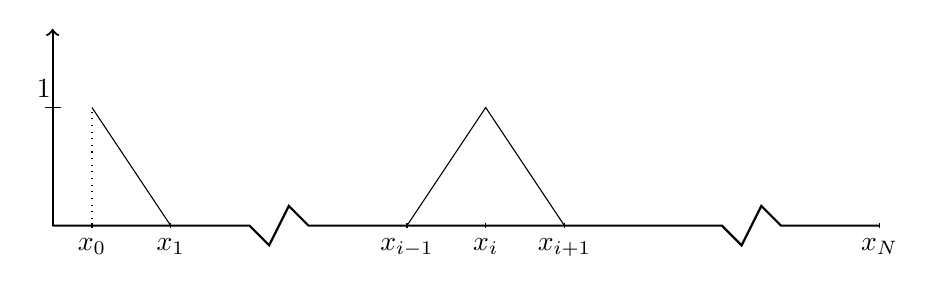
\begin{tikzpicture}

\draw[thick,->] (-0.5,0) -- (-0.5,2.5);
\draw (-0.6,1.5) -- (-0.4,1.5) node[anchor=south east] {$1$};
\draw[dotted] (0,0) -- (0, 1.5);
\draw[thick] (-0.5,0)--(2,0) -- (2.25,-0.25) -- (2.5,0.25) --(2.75,0)--(8,0) -- (8.25,-0.25) -- (8.5,0.25) --(8.75,0) -- (10,0) node[anchor=north west]{};

\draw (4,0) -- (5,1.5)--(6, 0) ;
\draw (4 cm,1pt) -- (4 cm,-1pt) node[anchor=north] {$x_{i-1}$};
\draw (5 cm,1pt) -- (5 cm,-1pt) node[anchor=north] {$x_{i}$};
\draw (6 cm,1pt) -- (6 cm,-1pt) node[anchor=north] {$x_{i+1}$};
\draw (0,1.5) -- (1,0);

\foreach \x in {0,1}
   \draw (\x cm,1pt) -- (\x cm,-1pt) node[anchor=north] {$x_\x$};

\draw (10 cm,1pt) -- (10 cm,-1pt) node[anchor=north] {$x_N$};

\end{tikzpicture}
\end{center}



\subsection{An Elliptical Model Problem} \label{subsec:Weak Formulation1}

Now we have defined the mathematical context let us solve a problem via the FEM. Take the stationary heat equation.

\begin{subequations} 
\label{eq:Steady Diffusion1} 
\begin{align}
-u'' &= f		\quad \quad  x \in [0, 1] \\  	
u(0) &= 0 \\
u(1) &= 0
\end{align}
\end{subequations}

The first step of solving this and any PDE by the FEM is to find a suitable weak formulation. This is given by multiplying both sides of the equation by a test function in the Sobolev space $v \in H^1_0(0, L)$.

\begin{equation*}
\int_0^L  u'' v  dx = \int_0^L  f v dx 	\quad \quad  dx \forall v \in H^1_0(0, L)
\end{equation*}

Integrating by parts on the left leads us to our weak formulation of \ref{eq:Steady Diffusion1}

\begin{problem}{Weak Formulation} \label{prob:Weak Formulation Elliptic}
\\Find $\quad u \in H^1_0(0, 1)$:
\begin{align*}
\int_0^L  u' v'  dx =   \int_0^L  f v dx  \quad \quad  \forall v \in H^1_0(0, L)
\end{align*}
$\forall v \in H^1_0(0, L)$
\end{problem}

Define 
\begin{equation*}
\int_0^L  u' v'  dx = a(u, v)  	
\int_0^L  f v dx  =  \ell(v)
\end{equation*}

This gives us the linear and bilinear form with can be used to show by \ref{app:LM} that $u$ exists and is unique. However, our test function has been chosen simply some function in the Sobolev space which has infinitely many functions defined within it and is described as infinite dimensional. 

To find the FEM approximation to \ref{eq:Steady Diffusion1} we look for a solution in a finite dimensional subspace of $V\subset H^1_0(0, L) $. The subspace we chose consists of continuous piecewise linear functions of defined on some given subdivision of $\Omega$. Then we can restate the weak formulation by the following:

Take the subdivision on $x \in \Omega$ in our model problem \ref{eq:Steady Diffusion1}. We subdivide the domain into N intervals $[x_k, x_{k+1}] \quad k=0, 1, ... , N-1$. This subdivision may not be regular and when later in this dissertation we begin seeking an adaptive solution will very rarely be regular. intervals may be referred to as elements and give the FEM its name.
\\
\begin{center}
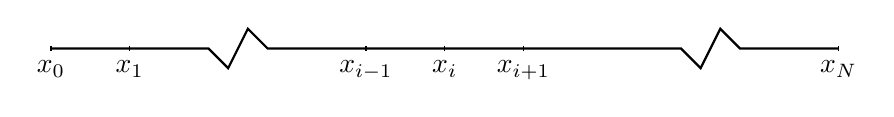
\begin{tikzpicture}



\draw[thick] (0,0)--(2,0) -- (2.25,-0.25) -- (2.5,0.25) --(2.75,0)--(8,0) -- (8.25,-0.25) -- (8.5,0.25) --(8.75,0) -- (10,0) node[anchor=north west]{};


\draw (4 cm,1pt) -- (4 cm,-1pt) node[anchor=north] {$x_{i-1}$};
\draw (5 cm,1pt) -- (5 cm,-1pt) node[anchor=north] {$x_{i}$};
\draw (6 cm,1pt) -- (6 cm,-1pt) node[anchor=north] {$x_{i+1}$};


\foreach \x in {0,1}
   \draw (\x cm,1pt) -- (\x cm,-1pt) node[anchor=north] {$x_\x$};

\draw (10 cm,1pt) -- (10 cm,-1pt) node[anchor=north] {$x_N$};

\end{tikzpicture}
\end{center}


\vspace{5mm} %5mm vertical space

\begin{problem}{FEM Approximation} \label{prob:Approx1}
Find $\quad u_h \in  V\subset H^1_0(0, 1) \quad : \\ a(u_h, v_h) =  \ell(v_h) \quad \forall v_h \subset V.$
\end{problem}

Now we can define our approximation $u_h$ to \ref{eq:Steady Diffusion1} by the ansatz:

\begin{equation} 
u_h(x) = \sum_{j=1}^{N(h)} U_j \cdot \phi_h(x) \label{eq:ansatz}
\end{equation}

With $U_j \: j = 1, ..., N(h)$ being constants to be determined. We can now rewrite \ref{prob:Approx1} by the following:

\begin{equation*}
\sum_{j=1}^{N(h)}U_j \: a( \,\phi_j(x),\, \phi_i(x)) = \ell(\,\phi_i(x)\,) 
\end{equation*}

This gives a system of linear equations with $a( \,\phi_j(x),\, \phi_i(x))$ an $N(h)\times N(h)$ matrix. 

\begin{equation} 
A_{ij} = \int_I \phi_i' \phi_j' dx \quad \quad \label{eq:stiff}
\end{equation}
\begin{equation}
F_i = \int_I  \, f\phi_i dx
\end{equation}
\vspace{2mm} %5mm vertical space
Hence the system $AU = F$.	


\subsection{Numerical Experiments} \label{subsec:results1}

First we take \ref{eq:Steady Diffusion1} a uniform partition with interval size $h$ such that.

\begin{subequations} 
\label{eq:Steady Diffusion1.1} 
\begin{align}
-u'' &= \pi^2 \cos(\pi x - 0.5 \pi)	\quad \quad  x \in [0, 1] \\  	
u(0) &= u(1) = 0 
\end{align}
\end{subequations}


\begin{figure}[h]
   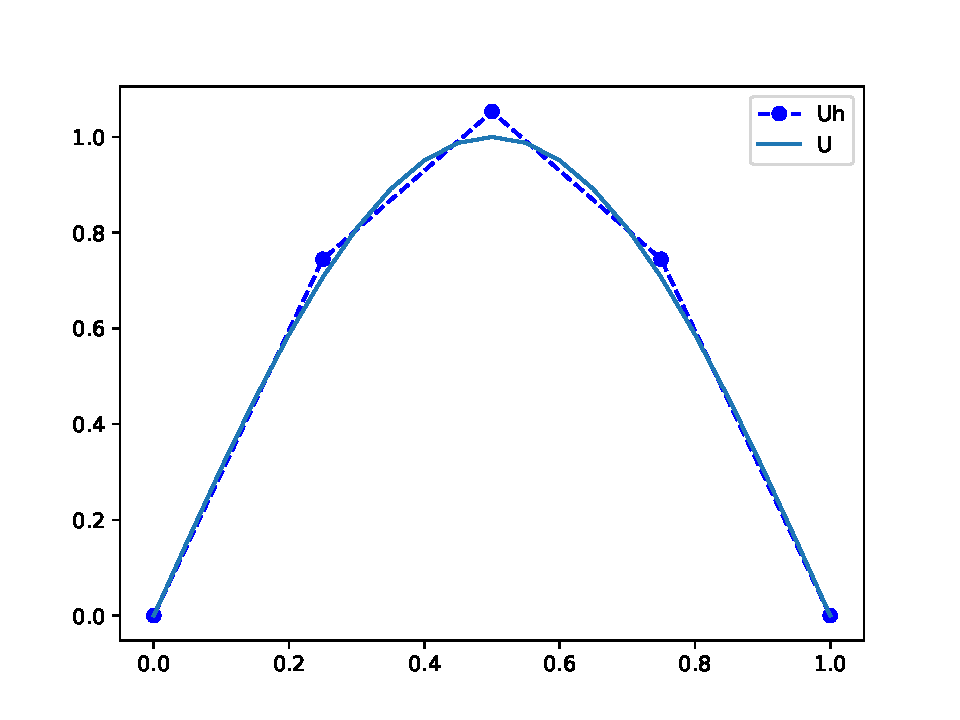
\includegraphics[width=0.5\textwidth]{EllipticPDE2.pdf}
   
 \label{fig:eliptic1}
\end{figure}



\begin{figure}[h!]
\begin{minipage}{0.48\hsize}
\begin{tabular}{ccc}
    \hline
     h & $\|u-u_h\|_{L_2(0,1)}$ & $\|u-u_h\|_{H^1(0,1)}$   \\ \hline
     $\tfrac{1}{4}$ & 0.0174706 &  0.511854   \\
     $\tfrac{1}{8}$ & 0.00413879 &  0.252837   \\
     $\tfrac{1}{16}$ & 0.00102063 &  0.12604   \\
	 $\tfrac{1}{32}$ & 0.000254283 &  0.0629727  \\
     $\tfrac{1}{64}$ & 6.3516e-005 &  0.0314805   \\

    \hline
  \end{tabular}
  \end{minipage}
  \hfill
    \begin{minipage}{0.48\hsize}
  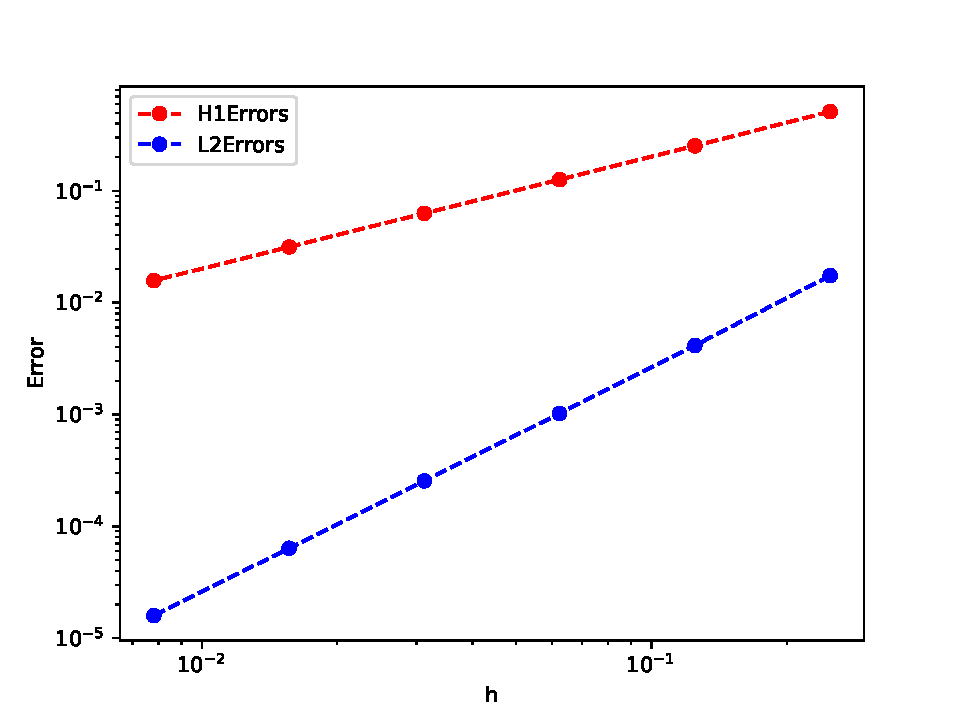
\includegraphics[width=0.9\textwidth]{EllipticPDE2Convergences.pdf}
  \label{fig:c}
\end{minipage}
    \end{figure}
    
\vspace{6mm}

We see smooth convergence in both of our chosen norms. In $\|u-u_h\|_{L_2(0,1)}$ the order of convergence is approximately $h^2$  and in $\|u-u_h\|_{H^1_0(0,1)}$ is approximately $h$. This tells us that the second term in $\|\cdot\|_{H^1_0(0,1)}$ related to the derivative is dominating and is order $h^2$.

This is a result that those with a knowledge of FEM may have been expecting. As we begin designing and investigating adaptive algorithms we will have to consider non-uniform meshes. The concept of interval width will remain important but from now on we also consider degrees of freedom (DOFs)which is the number of nodes in a given partition including the boundary nodes. Take following adjustment of \ref{eq:Steady Diffusion1} and its approximation without uniform intervals.

	%the righthandside may be wrong. Needs checking 
\begin{subequations} 
\label{eq:Steady Diffusion2} 
\begin{align}
-u'' &= \pi^2 \sin( \pi x)		\quad \quad  x \in [0, 1] \\  	
u(0) &= 0 \\
u(1) &= 1
\end{align}
\end{subequations}


\begin{figure}[h]
   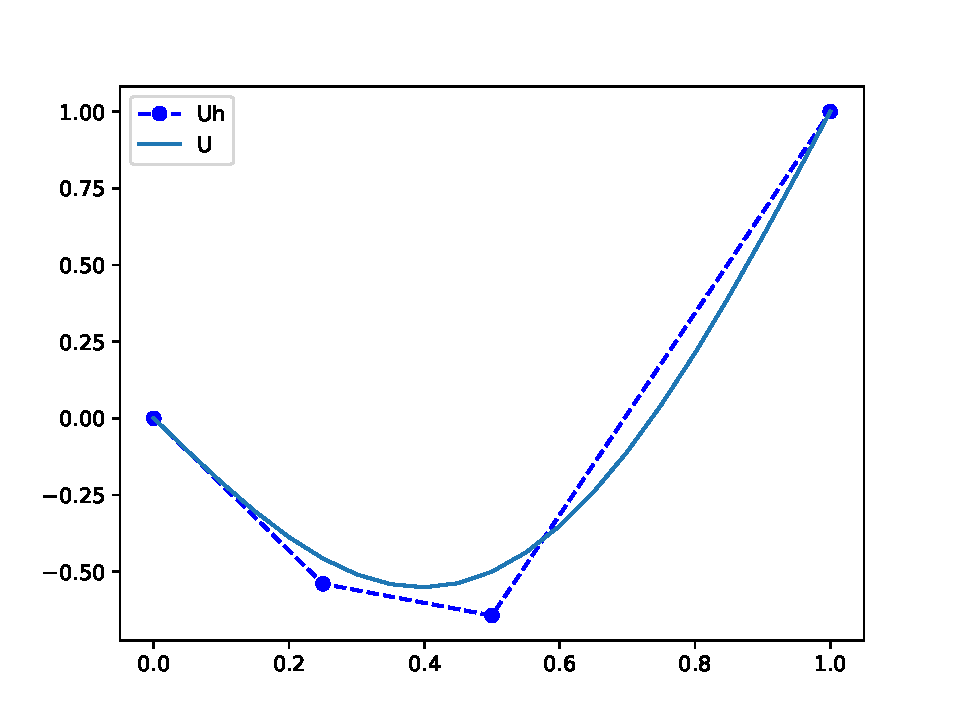
\includegraphics[width=0.5\textwidth]{EllipticPDE1_hi.pdf}
 \label{fig:eliptic1}
\end{figure}


\begin{figure}[h!]
\begin{minipage}{0.48\hsize}
\begin{tabular}{ccc}
    \hline
     DOFs & $\|u-u_h\|_{L_2(0,1)}$  & $\|u-u_h\|_{H^1(0,1)}$   \\ \hline
     $4$ & 0.0776354  & 0.825144   \\
     $7$ & 0.0170398  & 0.40185   \\
     $13$ & 0.00411272  & 0.199548   \\
	 $25$ & 0.00101902  & 0.0996014 \\
    $49$ & 0.000254182  & 0.0497791   \\
    \hline
  \end{tabular}
  \end{minipage}
  \hfill
    \begin{minipage}{0.48\hsize}
  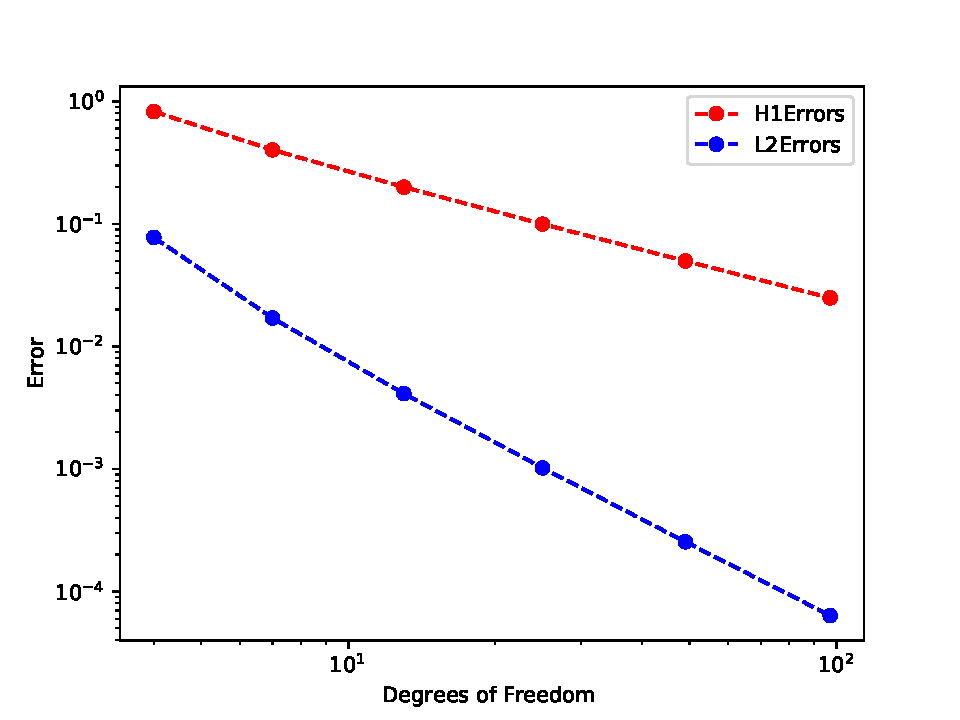
\includegraphics[width=0.9\textwidth]{EllipticPDE1Convergences.pdf}
\end{minipage}
    \end{figure}
    
\vspace{6mm}

We see the hoped for convergence with respect to the degrees of freedom. As we perhaps expected we see the order of convergence in the $L_2$ and $H_1$ norms of $n^{-2}$ and $n^{-1}$ respectively where n represents the degrees of freedom. 

\subsection{Implementation} \label{subsec:Implementation1}

It is evident that all the matrices that arise from the one dimensional FEM are tridiagonal. This is important as there are efficient algorithms available for solving tridiagonal systems. This is an ideal opportunity to create a data structure to store these matrices and associate the any methods that we would like to use throughout the project. To do this we define our base class for tridiagonal matrices and define within it a method "Matrix Solver" which implements the Thomas algorithm. One possible declaration of this design pattern is given below and the full implementation is given in appendix \ref{app:Tridiag}:

\begin{lstlisting}[language=C++]
class TriDiagMatrix{
public:
    void MatrixSolver( std::vector<double> f,
         std::vector<double> &x );

protected:
    std::vector<double> mpDiagonal;
    std::vector<double> mpLowerDiag;
    std::vector<double> mpUpperDiag;
};
\end{lstlisting}



The obvious advantage of a similar declaration is not only the efficiency of the storage and the methods but also the readability, polymorphism and the ease with which the code can then be tested. Once module tests have been run and effectiveness established we can derive any specific matrices we need from the above base. The first derivation we make is for \ref{eq:stiff} also called the Stiffness matrix. This class reads a specific subdivision of the domain and sets the Stiffness matrix accordingly.

\begin{lstlisting}[language=C++]
class StiffnessMatrix: public TriDiagMatrix{
public:
    void BuildStiffnessMatrix ( SpaceMesh& smesh ); };

\end{lstlisting}

With these tools we can present the code which produced \ref{fig:eliptic1}. The major point we emphasise here is readability and code safety. As we move to solving parabolic PDEs in the next section this modular approach will allow our code to scale.

\begin{lstlisting}[language=C++]
void StationaryHeatEquation(){
StiffnessMatrix ( mpsmesh );
buildfvec( mpsmesh)
stiff.MatrixSolver( f_vec, U );
PrintVector(U);
}
\end{lstlisting}

\subsection{Boundary Conditions} \label{BCs}
We have not yet discussed in detail the implementation of boundary conditions. This has been done in \ref{prob:Weak Formulation Elliptic} by choosing $H^1_0(0, L)$ for our homogeneous dirichlet boundaries.
In general we use this "trick" in this dissertation when defining the weak formulation. This is done to avoid delving into the detail of choosing the correct solution space for our solution which is outside of the remit of this dissertation.

However, in practise one of the major advantages of the FEM is the ease with which more complicated boundary conditions can be implemented. One method for doing this is a penalty method of implementing Robin boundary conditions and using parameters to approximate non-homogeneous dirichlet conditions. Neumann boundaries can also be implemented in this way.

A detailed account of implementing Robin boundary conditions with parameters is given in \cite{larson2013finite}. Where our examples extend to PDEs with non-homogeneous boundary conditions this is what we have done. 

\clearpage

\section{Discretising the Time Dependent Problem} \label{sec:Time dependent}



Now that we have built some foundations by solving an elliptical PDE ref{eq:Steady Diffusion1} we can consider parabolic Heat Equation. The steps involved in solving the parabolic version are:

\begin{enumerate}
\item We discretise in space as before, however we adjust the solution space to consider our basis functions for a sequence of specific times that vary in x. This can be thought of loosely as a sequence of elliptical problems.  

\item Creating the subdivision of our domain $\Omega$ in both space and time. Replace our infinite dimensional function space by a finite dimensional subspace. We see that we can use the same basis functions.

\item We discretize in time using a Finite Difference method -in our case the Implicit Euler method.


\item We solve the resulting system of equations at the given time steps
\end{enumerate}

Once we have carried out these steps we will perform some numerical experiments and convergence analysis and then close the chapter with a discussion of mesh design and related data structure. "Meshing" is the art-form that underpins the adaptive FEM and so merits close attention. 



\subsection{Semi-discrete Problem} \label{subsubsec:Semi-discreet}

To describe the semi-discrete problem we will take the following model problem. 


\begin{subequations} 
\begin{align}
  \dot{u} - u'' = & f \quad x \in [0, L], \quad t \in (0, T]  \\ \label{eq:Simple Heat}
  u(0, t) & = u(L, t) = 0\\
  u(x, 0) & = u_0(x)   
\end{align}
\end{subequations}

Multiplying $\dot{u} - u'' = f$ by a test function  $v \in H^1_0(0, L)$  on both sides. 

\begin{equation*}
  \int_0^L \dot{u} v dx  - \int_0^L  u'' v  dx =   \int_0^L  f v  dx   
\end{equation*}
\vspace{1mm}

Integrating by parts yields:

\begin{equation*}
  \int_0^L \dot{u} v dx  + \int_0^L  u'' v  +u(0)v(0) - u(L)v(L) dx =   \int_0^L  f v  dx   
\end{equation*}

\begin{equation*}
  \int_0^L \dot{u} v dx +  \int_0^L  u' v'  dx =   \int_0^L  f v  dx    
\end{equation*}
\vspace{1mm}

The weak formulation of our problem is now given by:

\begin{problem}{Weak Formulation} \label{prob:weak2}\\
Find $\: u(\cdot, t) \in H^1_0(0, L)$:
\begin{align*}
	(&\dot{u}(\cdot, t), v) + a(u(\cdot, t), v) = (f(\cdot, t), v)\\
	(&u(\cdot, 0), v) = (u_0, v)
\end{align*}
$\forall v \in H^1_0(0, L)$
\end{problem}
Here,
\begin{align*}
 a(w, v)  = \int_0^L  w' v'  dx 
 (w, v) = \int_0^L  w v  dx 
\end{align*}


To find our approximation define a mesh on $[0, 1] \times [0, T]$.\\

\begin{center}
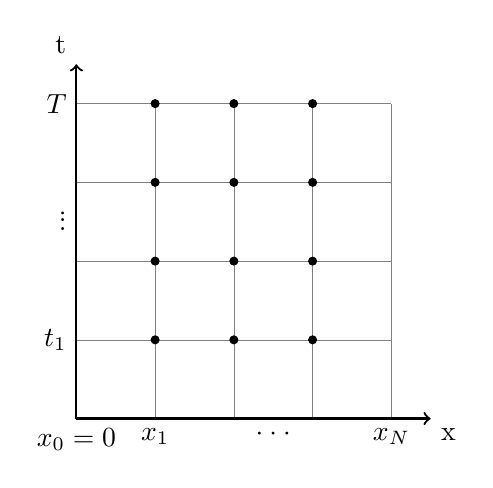
\begin{tikzpicture}

\draw[step=1cm,gray,very thin] (0,0) grid (4,4);
\foreach \x in {1,2,3}
	\foreach \y in {1, 2, 3, 4}
    	\filldraw (\x,\y) circle (0.05cm);
    	
\draw[thick,->] (0,0) -- (4.5,0) node[anchor=north west] {x};
\draw[thick,->] (0,0) -- (0,4.5) node[anchor=south east] {t};
    	
\draw (0,4) node[anchor=east] {$T$};
\draw (0,0) node[anchor=north] {$x_0=0$};
\draw (1,0) node[anchor=north] {$x_1$};
\draw (2.5,0) node[anchor=north] {$\cdot \cdot  \cdot$};
\draw (4,0) node[anchor=north] {$x_N$};
\draw (0,1) node[anchor=east] {$t_1$};
\draw (0,2.5) node[anchor=east] {$\dot{:}$};

\end{tikzpicture}
\end{center}

Let the partition on the space mesh be $0 = x_0< x_1< ...< x_N = 1$ with intervals\\ $h_i = x_i - x_{i-1}$. Let the time partition be $0 = t_0< t_1< ...< t_M = T$ time steps $\Delta t_j = t_j - t_{j-1}$. For both space and time we allow the intervals to vary.

Let $V\subset H^1_0(0, 1)$ denote the set of all continuous piecewise linear functions defined on the space mesh that are zero on the boundaries $x=0$ and $x=1$. 

\subsubsection{Implicit Euler} \label{subsubsec:Implicit Euler}

\ref{weak2} is the a space discrete problem, sometimes referred to as the semi-discreet problem but we now need to discretise in time to be able to find an approximation to the solution. We will use Finite Differences to discretise in time and we will choose the Implicit Euler method. 


\begin{problem}{Implict Euler Method} \label{eq:Implicit Euler}
\\Find $u_h^{m+1} \in V \quad 0 \leq m \leq M-1$
\begin{align*}
\Big(\frac{u_h^{m+1} \, - \, u_h^{m}}{\Delta t}, v_h \Big) +\: a(u_h^{m+1}, v_h) \quad=&\quad (f(\cdot, t^m), v_h) \\
(u^{0}_h - u_0, v_h)\quad  =& \quad0 \quad \forall v_h \in V
\end{align*}
\end{problem}
%a(u_h^m, v_h) =& (f(\cdot, t^m), v_h) \\
%{u^{0}_h - u_0, v_h) =& 0 \quad \forall v_h \in V

We can therefore rewrite the system as:

\begin{align*}
( u_h^{m+1} \, v_h)  + \: \Delta t a(u_h^{m+1}, v_h) \quad=\quad (u_h^{m}, \, v_h ) \:+\: \Delta t(f(\cdot, t^m), v_h) \\
\quad \forall v_h \in V \quad 0 \leq m \leq M-1 \\
\end{align*}

	with
\begin{equation*}
(u^{0}_h) \quad  = \quad u_0, v_h \quad \forall v_h \in V
\end{equation*}

Then as in section \ref{sec:FEM} we choose the FEM basis function and use the ansatz \ref{eq:ansatz} to form a system of equations at each time.

\subsection{Numerical Experiments} \label{subsec:results2}

\subsubsection{A Convergence Study} \label{subsec:convegence2}

Take the model problem \ref{eq:Simple Heat} without a source function and thermal diffusivity $\pi^{-2}$

\begin{subequations} 
\begin{align}\label{eq:Simple Heat1}
  \dot{u} - \pi^{-2} \: u'' = &\: 0 \quad x \in [0, L], \quad t \in (0, 1]  \\ 
  u(0, t) & = u(1, t) = 0\\
  u(x, 0) & =  6sin( \pi x)
\end{align}
\end{subequations}

\begin{figure}
\caption{The analytic solution to \ref{eq:Simple Heat1} shows the diffusion of heat over time in our system}
 \label{fig:Heat1}
   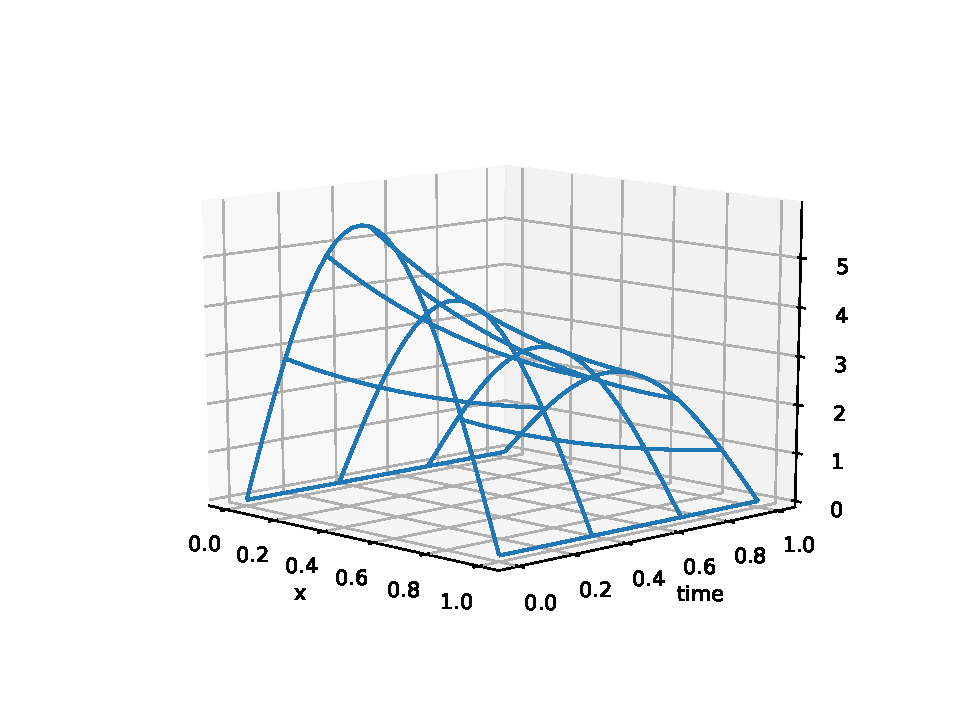
\includegraphics[width=0.7\textwidth]{Heat1angle.pdf}
\end{figure}



\begin{figure}[h]
\caption{The plots of our approximation appear to follow our analytic solution \ref{fig:Heat1} }
\begin{minipage}{0.49\hsize}
  \label{fig:Heat1approx}
   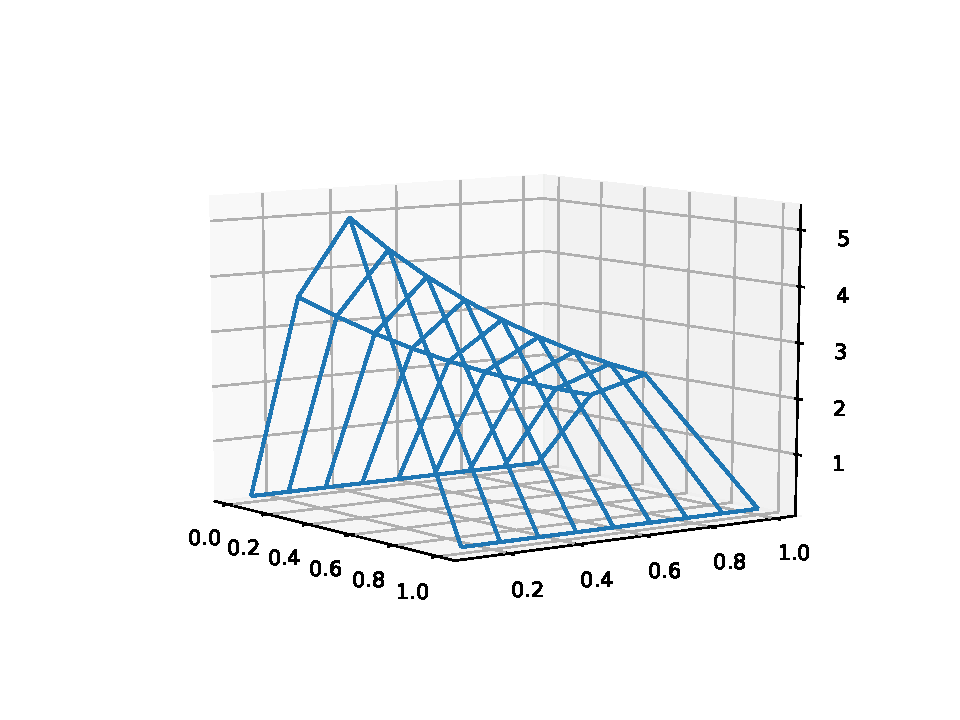
\includegraphics[width=1.2\textwidth]{firstPDE3d.pdf}
  \end{minipage}
  \hfill
    \begin{minipage}{0.49\hsize}
    \vspace{5mm}
    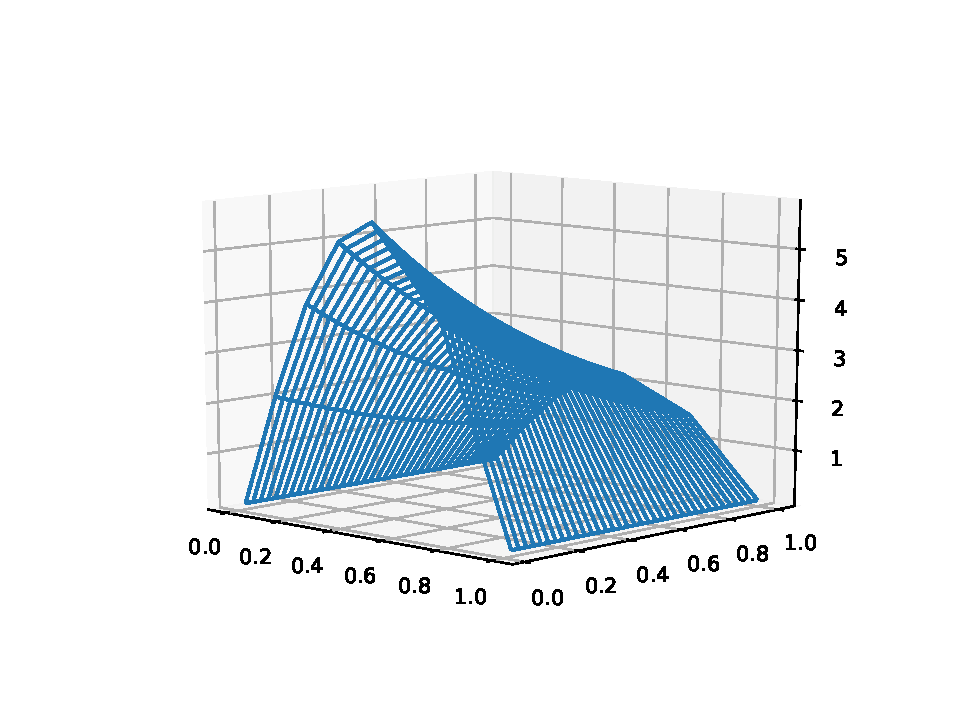
\includegraphics[width=1.2\textwidth]{firstPDE3dfine.pdf}
\end{minipage}
    \end{figure}

To study the convergence of our solution we set $\Delta t = n^{-2} $ for time step of size $\Delta t$ and degrees of freedom $n$. We then study the solution at the final time for various numbers of degrees of freedom. 

\begin{figure}[h!]
\caption{We can see the approximation converging to the true solution in the final time}
\begin{minipage}{0.49\hsize}
   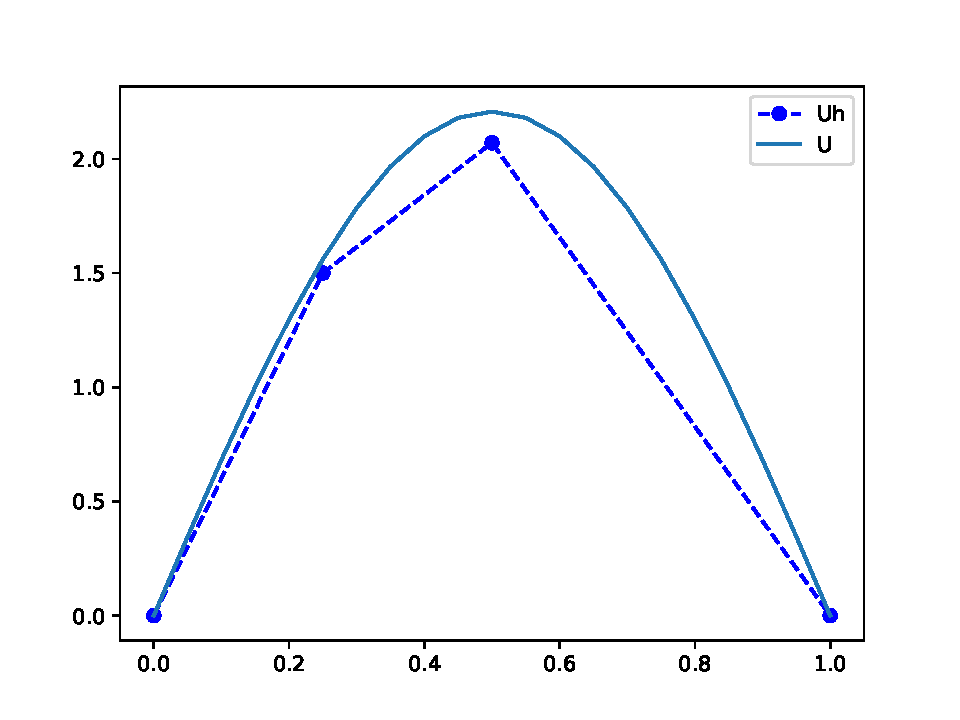
\includegraphics[width=0.95\textwidth]{OriginalPDEcoarse.pdf}
  \end{minipage}
  \hfill
    \begin{minipage}{0.49\hsize}
    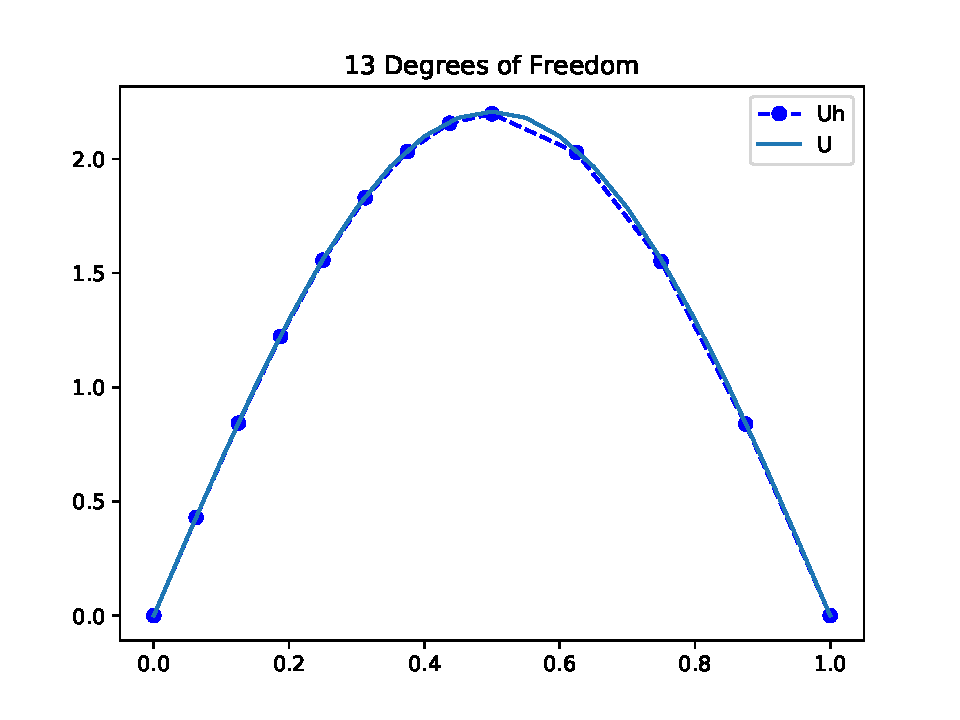
\includegraphics[width=0.95\textwidth]{OriginalPDEfine.pdf}
  \label{fig:heat1_final}
\end{minipage}
    \end{figure}
    
    
    
\begin{figure}[h!]
\begin{minipage}{0.48\hsize}
\begin{tabular}{ccc}
    \hline
 DOFs & $\|u-u_h\|_{L_2(0,1)}$  & $\|u-u_h\|_{H^1(0,1)}$  \\ \hline
 $4$ & 0.304466 & 1.74657   \\
$7$ & 0.0918245 & 0.883062  \\
$13$ & 0.0231464 & 0.439949  \\
$25$ & 0.00575675 & 0.219779 \\
$49$ & 0.00143142 & 0.109867  \\
 \end{tabular}
  \end{minipage}
  \hfill
    \begin{minipage}{0.48\hsize}
  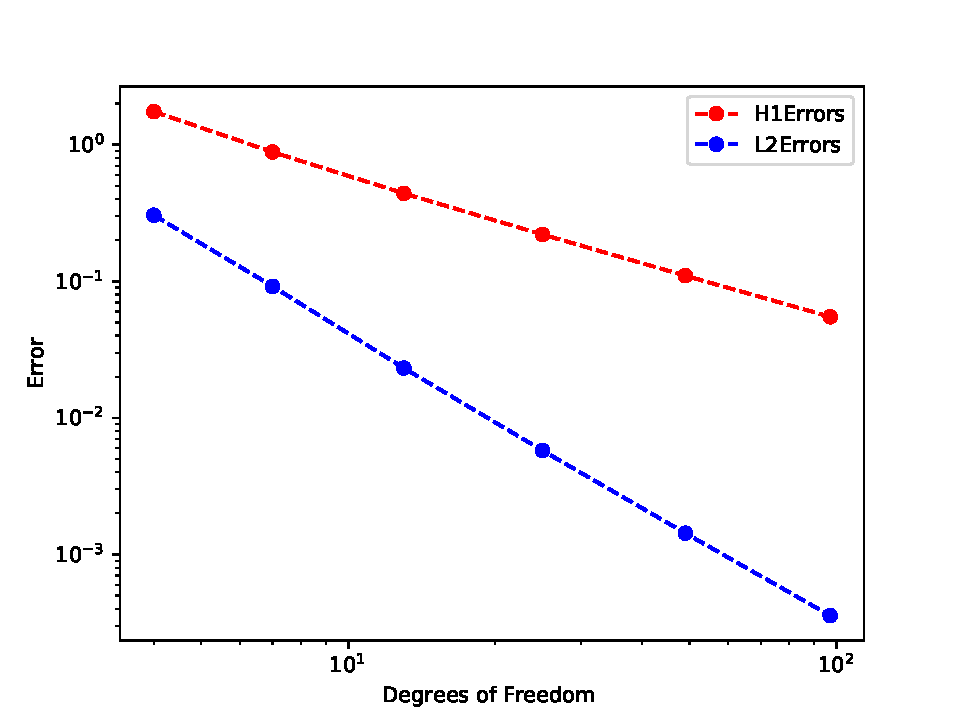
\includegraphics[width=0.9\textwidth]{ParabolicConvergencesOriginal.pdf}
  \label{fig:c}
\end{minipage}
    \end{figure}

We have convergence of approximately order $n^{-2}$ in the $L_2$ norm and order $n^{-1}$ in the $H^1$. This is perhaps what we expected from the stationary example however the choice $\Delta t = n^{-2} $ was important to find this convergence.


\subsubsection{Another Convergence Study} \label{subsec:convegence2}

 We will now justify this choice numerically by looking at convergence for a different choice of $\Delta t$. Consider again the model problem \ref{eq:Simple Heat} with adjusted boundary conditions and initial data. This time set $\Delta t = n^{-1} $.

 

\begin{subequations} 
\begin{align}\label{eq:Simple Heat2}
  \dot{u} - \pi^{-2} \: u'' = &\: 0 \quad x \in [0, L], \quad t \in (0, 1] \\ 
  u(0, t) & = 0  \quad u(1, t) = 1\\
  u(x, 0) & =  2sin(2 \pi x) +x
\end{align}
\end{subequations}

\begin{figure}[h!]
\caption{The analytic solution to \ref{eq:Simple Heat2} shows the diffusion of heat over time in our system}
 \label{fig:Heat2}
   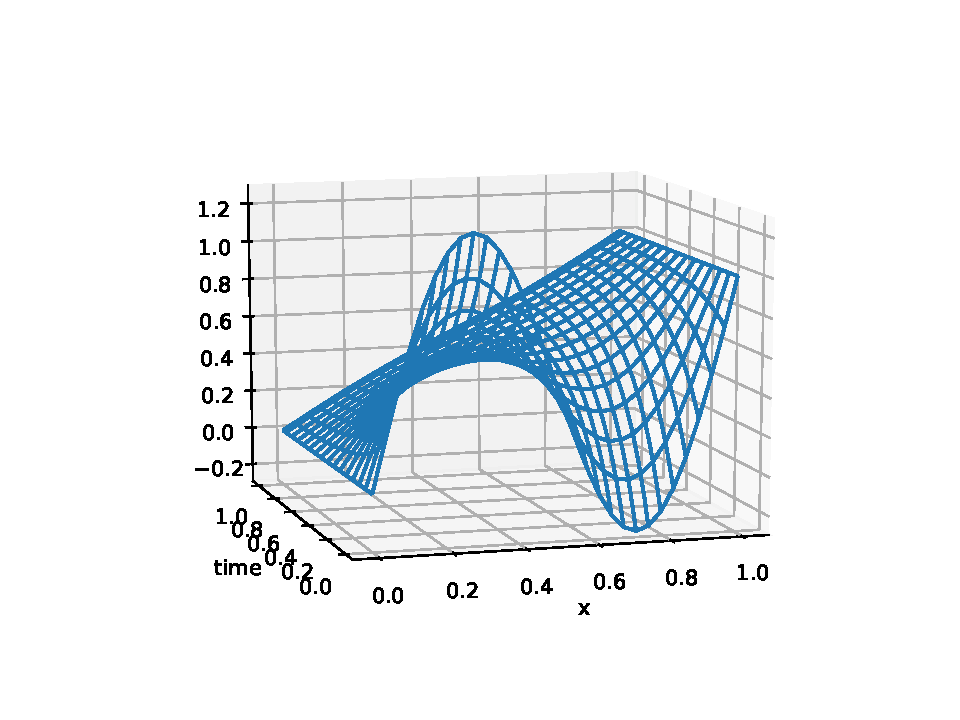
\includegraphics[width=0.8\textwidth]{Heat2.pdf}
\end{figure}


\begin{figure}
\caption{We see that the coarse approximation is quite different from figure \ref{eq:Simple Heat2} which is a symptom of the mesh we have used. However, the fine approximation begins to approach the expected shape}
\begin{minipage}{0.49\hsize}
   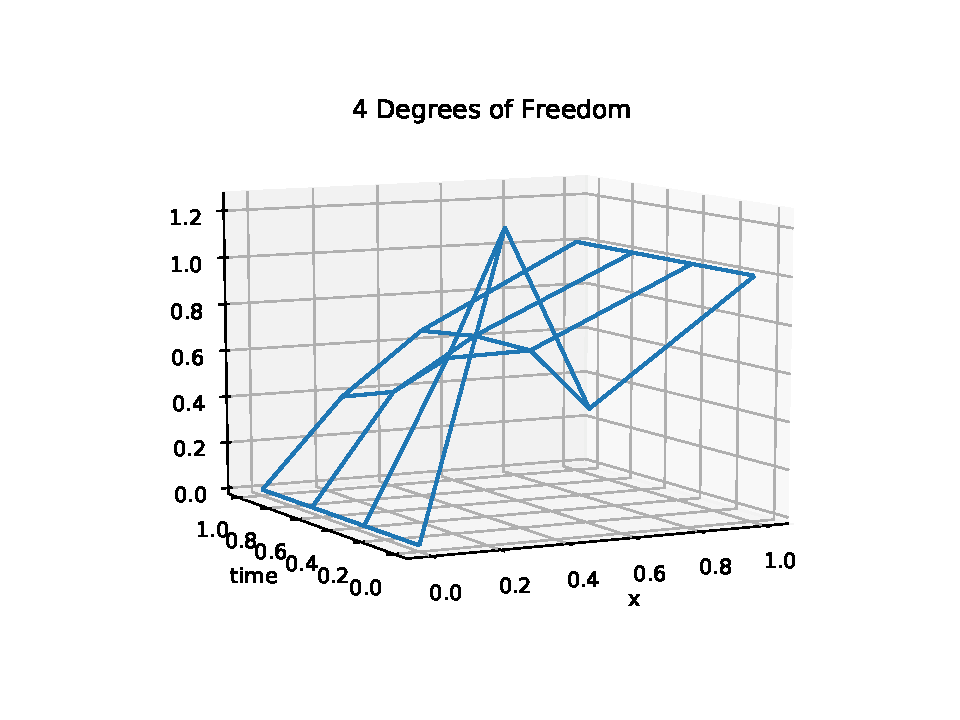
\includegraphics[width=1.2\textwidth]{CAMQ2delta_t_nCoarse.pdf}
  \end{minipage}
    \begin{minipage}{0.49\hsize}
    \vspace{5mm}
    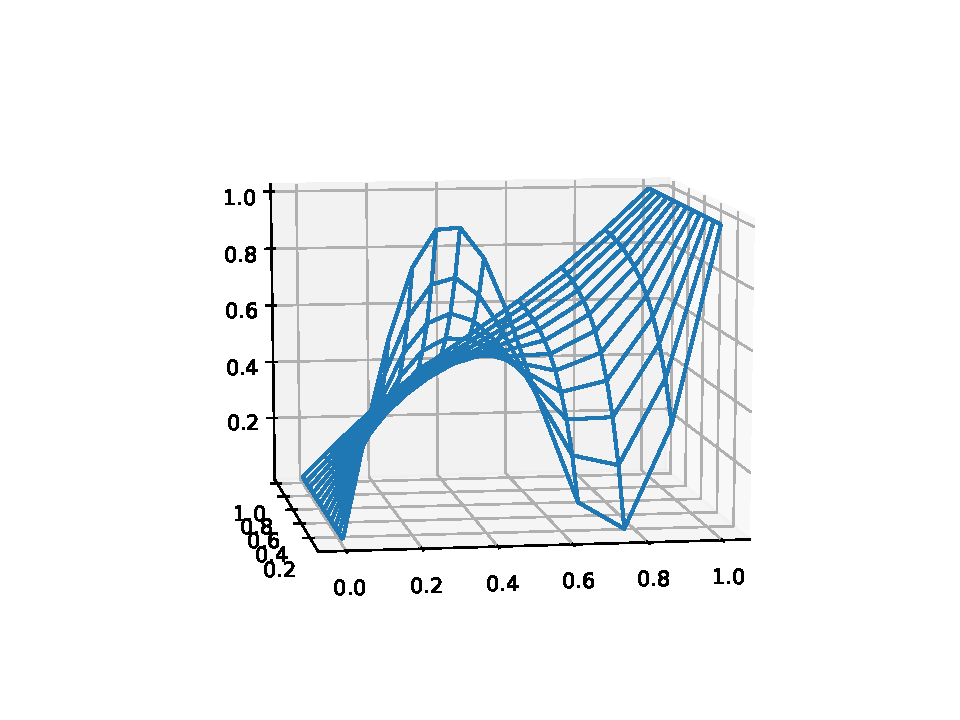
\includegraphics[width=1.2\textwidth]{CAMQ2delta_t_nFine.pdf}
  \label{fig:c}
\end{minipage}
    \end{figure}
    

\begin{figure}
\caption{We have the appearance of convergence in the final time as well}
\begin{minipage}{0.49\hsize}
   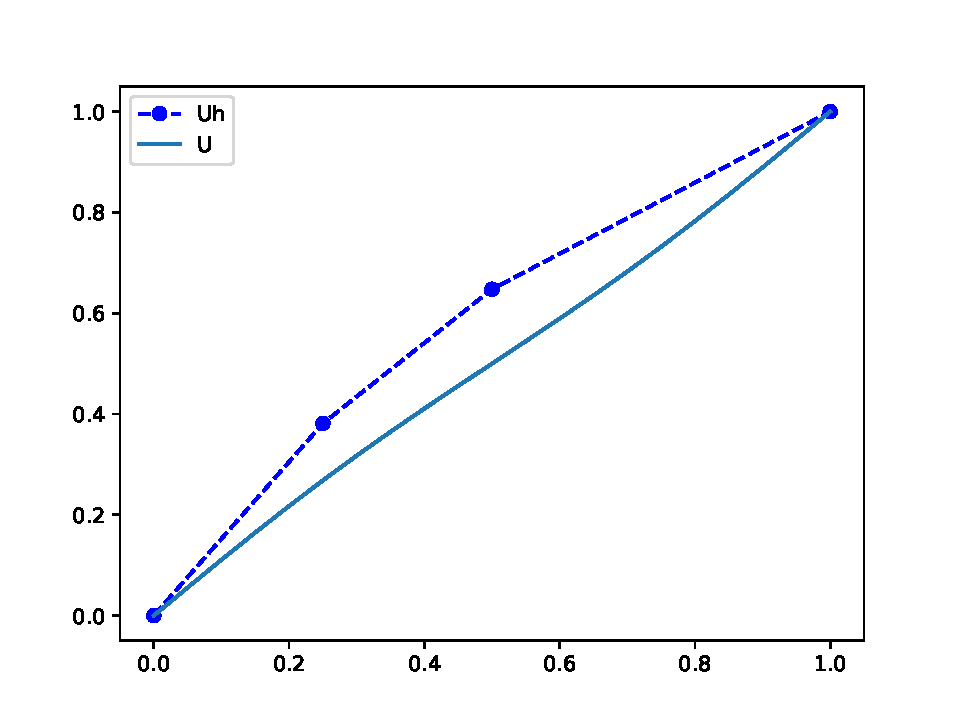
\includegraphics[width=0.95\textwidth]{Heat2FinalTimeCoarse.pdf}
  \end{minipage}
  \hfill
    \begin{minipage}{0.49\hsize}
    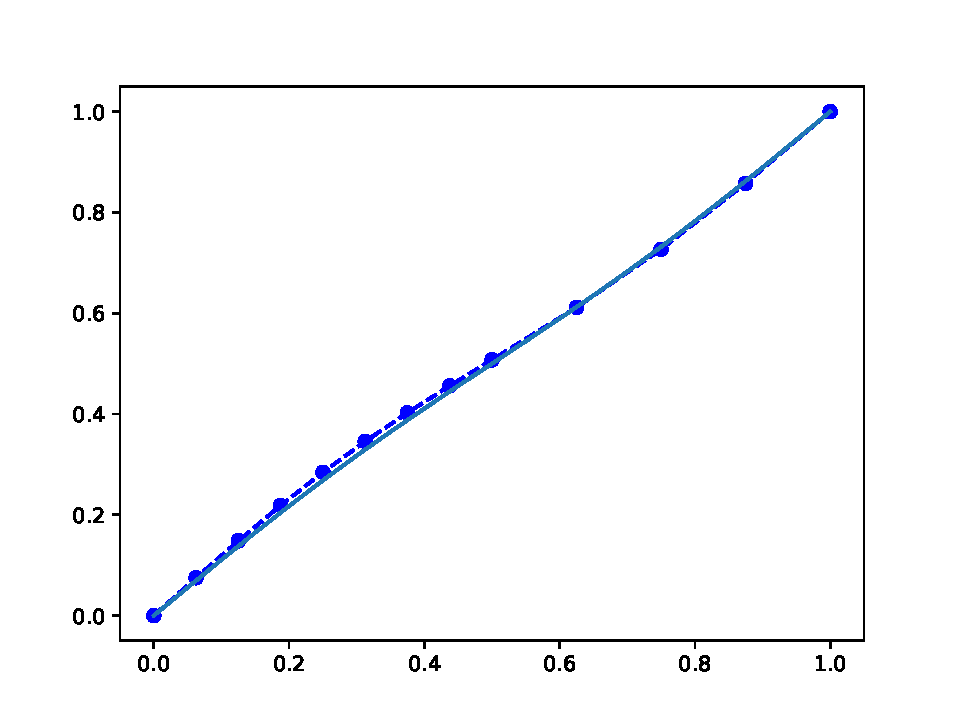
\includegraphics[width=0.95\textwidth]{Heat2FinalTimeFine.pdf}
  \label{fig:heat2_final}
\end{minipage}
    \end{figure}
    

\begin{figure}[h!]


 \label{fig:Heat2_convergence}
   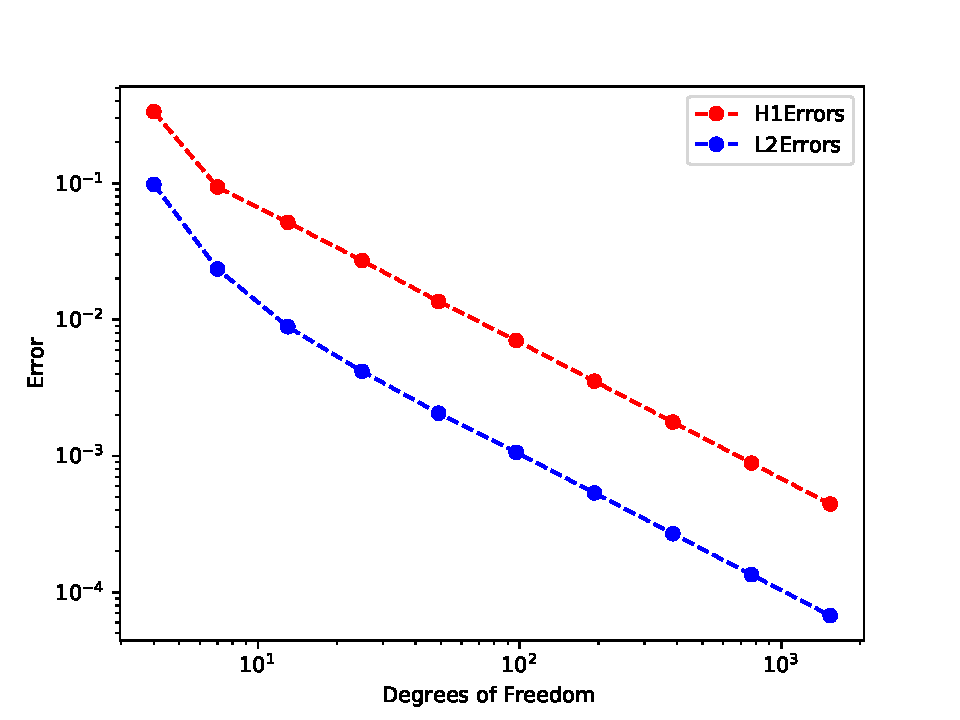
\includegraphics[width=0.7\textwidth]{ConvergencesCAMQ2delta_t_n.pdf}
   
\caption[my caption] {When we explore the approximations in the $L_2$ and the $H_1$ norms we see some limitations of our choice $\Delta t = n^{-1} $. This is because both the FEM and the Implicit Euler method incur errors. The FEM converges order $L_2$ and $H_1$ norms of $n^{-2}$ and $n^{-1}$ as we showed in subsection \ref{subsec:results1}. The implicit Euler converges order $\Delta t$ so the convergence of the fully discreet problem is order $\Delta t + n^{-1}$ in the $L_2$ norm and $\Delta t + n^{-2}$ in the $H^1$ norm.

We can therefore see that for the choice $\Delta t = n^{-1} $ the term $\Delta t $ limits the order of convergence. This is undesirable as in this dissertation we are primarily interested in the efficiency of the adaptive algorithm with respect to degrees of freedom. From now on in this dissertation we set  $\Delta t = n^{-2} $ as in subsection \ref{subsec:convegence2} so that we can retain a focus on the quality of the solution wrt to DOFs.}
\end{figure}



\clearpage
\subsection{Implementation} \label{subsubsec:Implementation}

"Meshing" is the important art-form on which the computer implementation of the FEM depends. There are entire software packages available to carry out the creation and manipulation of mesh structures and it would therefore benefit any FEM project to either design there own data-structures or implement an existing mesh package. 

An important question when designing the data-structure and class inheritance structure is the relationship between the time-steps and the space nodes. In our space nodes are free to vary at a given time step however the time steps are the same when considered from a given node. This seems to both invite and discourage the creation of a single base class from which to derive meshing in space and time. Much of the functionality of each is shared but much differs:

\begin{lstlisting}[language=C++]
class SpaceMesh
{
public:
    void CopySpaceMesh (const SpaceMesh& oldSpaceMesh);
    void BisectIntervals (std::vector<int> &intervalsForBisection);
    void CommonMesh( SpaceMesh& firstmesh, SpaceMesh& secondmesh );
    double TestFunctions(int nodeIndex, double x);
    bool Contained (double my_var );
protected:
    std::vector<double> mpSpaceNodes ;
};

class TimeMesh
{
public:
    void CopyTimeMesh (const TimeMesh& oldTimeMesh);
    void GenerateTimeMesh ( std::vector<double> TimeNodes );
    void BisectInterval (int lowerIndex, int upperIndex);
protected:
    std::vector<double> mpTimeNodes;
};

\end{lstlisting}

The question of how to structure inheritance in FEM meshes is in this case restricted to the one dimension and may seem abstract at the beginning of a project. However, there are many utility style functions i.e. adding a node or copy construction which could be simplified if there was an abstraction which could be justified rigorously. The danger of a heuristic abstraction pattern is that one of the child classes have access to a function which cannot be used safely or that the program not scale because of access restriction to prevent unsafe function calls. Though we found it prudent to separate time and space meshes some future work may under cover a good design pattern to combine them under a base class.
The program file for some of the important methods in SpaceMesh class are included in appendix \ref{app:space mesh}. The full header file for TimeMesh is also included for consideration in appendix \ref{app:time mesh}. However, he program files are not included as most are just combinations of fairly simple algorithms performed on dynamic arrays. 

\newpage

\section{A Posteriori Error Analysis} \label{sec:Errors}

When a continuous problem is discretised by Finite Element Methods and approximated numerically an error is incurred. Some knowledge about the error is available in advance of the implementation of a specific FEM approximation. This type of error analysis, so called a priori, is valuable for the analysis of convergence and other proofs that may be important about an FEM scheme in general. Although useful in these applications it is rare that an a priori error estimate accurately quantifies the error present in a numerical solution. As such in a practical context the a priori error cannot be used to indicate the quality of a solution in a practical sense. 

In contrast, a posteriori error analysis uses the computed numerical solution $u_h$ itself to estimate and quantify the true the error. Where a posteriori error estimates are available and accurate this has the obvious advantage that it describes the error in the approximation without the need for an analytical solution. This replaces the heuristics and guess work that had previously guided the error analysis of the FEM approximation in settings where no analytical solution was available \cite{ainsworth65001posteriori}. 

Since the initial pioneering methods of Babuska \cite{babuska1978posteriori} \cite{babuska1981posteriori} in this field many a posteriori error methods have been presented. Many of these have been shown to be effective in context. The emphasis in the literature has moved now from the discovery of new a posteriori estimates to the testing of the limitations of existing a posteriori estimates. All this is done primarily with the goal of validating the extensively used self-adapting FEM packages.

\subsection{Gradient Recovery} \label{subsubsec:KK}

The FEM provides an approximation to an unknown function, however the gradient of the function may also be of particular interest also. The gradient in the approximation is discontinuous over element boundaries but can be smoothed out by post-processing. In fact under certain circumstances the smoothed gradient is much closer to the gradient of the true solution \cite{ainsworth65001posteriori}. This leads fairly directly to one of the simpler a posteriori error estimates which is achieved by comparison of the approximated gradient before and after this post-processing.

Consider again the steady state one dimensional Heat Equation \ref{eq:Steady Diffusion1} and here restating its weak formulation for ease.


Find $\quad u \in H^1_0(0, 1)$:
\begin{align*}
\int_0^L  u' v'  dx =   \int_0^L  f v\, dx  \quad \quad  \forall v \in H^1_0(0, L)
\end{align*}
$\forall v \in H^1_0(0, L)$

With
\begin{equation*}
\int_0^L  u' v'  dx = a(u, v)  	
\end{equation*}

It is clear that the bilinear form is symmetric i.e.  a(w, v) = a(v, w) and it can be shown that it is coercive as described in the Lax Milgram theorem \ref{app:LM}. Hence, $a(w, v)$ is an inner product $(w, v)_a$ on  $H^1_0(0, L)$.

We can then define the associated energy norm.

\begin{equation}
\|w\|_a = |(w, w)_a|^\frac{1}{2}
\end{equation}

If we measure the true error in the energy norm we get.

\begin{equation}
\|u-u_h\|_a^2 = \int_0^L  u' - u_h'  dx
\end{equation}

Which is the $L_2$ norm of of the difference between the gradient and the approximated gradient which is sometimes called the $H^1$ semi-norm.

If we had the true gradient we would now be able to measure the true error in the energy norm. As that is unavailable we will use an estimate of the true gradient which will be obtained by some suitable post- processing of the FEM approximation to the solution. Let the post processed FEM approximated gradient be denoted by $G_h(u_h)$ then the error indicator for \ref{eq:Steady Diffusion} is given by:

\begin{equation}
\eta^2 = \int_0^L  |G_h(u_h) - u_h|^2  dx
\end{equation}

Clearly there are as many different error indicators as there are ways of processing the FEM approximation to the gradient. To describe one way we consider an FEM approximation to an elliptical.

\begin{center}
\begin{tikzpicture}

\draw[thick,->] (0,0) -- (10,0);
\draw[thick,->] (0,0) -- (0,2.5);

\draw[blue,thick,dashed] (0,0) -- (2,2.2) -- (4,2.8) -- (8,0);

\end{tikzpicture}
\end{center}

The gradient of this approximation is a discontinuous step-like function, undefined at the nodes of the space mesh.

\begin{center}
\begin{tikzpicture}

\draw[thick,->] (0,2) -- (8,2) ;
\draw[thick,->] (0,0) -- (0,6) ;

\draw[blue,thick] (0,3.1) -- (2,3.1);
\draw[blue,thick] (2,2.3) -- (4,2.3);
\draw[blue,thick] (4,1.3) -- (8,1.3);

\filldraw (2,2.7) circle (2pt);
\filldraw (4,1.8) circle (2pt);


\end{tikzpicture}
\end{center}

Intuitively a better approximation would be given by a function defined in the whole domain. A simple but logical one to use could be a continuous piecewise linear function as we have the architecture in our code to linearly interpolate sets of points. We take the midpoint of the FEM approximated gradient where currently our gradient is undefined and hence where we expect post-processing to have the greatest effect. 

More formally results exist to support this choice. In the case of a uniform partition the "super-convergence" of the centroid of two elements is shown by \cite{zlamal1978superconvergence}. Though true "super-convergence" may not be assured on our more general partition our method nonetheless should be an improvement on the untreated gradient. 

We also need to decide what to do with the elements at each side as our current method will not produce points for on the boundaries. We will choose to have the interpolant take the value of the gradient in the centre of the elements.



\begin{center}
\begin{tikzpicture}

\draw[thick,->] (0,2) -- (8,2) ;
\draw[thick,->] (0,0) -- (0,6) ;

\draw[blue,thick] (0,3.1) -- (2,3.1);
\draw[blue,thick] (2,2.3) -- (4,2.3);
\draw[blue,thick] (4,1.3) -- (8,1.3);

\filldraw (1,3.1) circle (2pt);
\filldraw (2,2.7) circle (2pt);
\filldraw (4,1.8) circle (2pt);
\filldraw (6,1.3) circle (2pt);

\draw[blue,thick,dashed] (0,3.5) --(1,3.1) --(2,2.7) -- (4,1.8)  -- (6,1.3) -- (8,0.8);


\end{tikzpicture}
\end{center}

\subsection{Effectivity Index} \label{subsec:results3}

In fact this method gives a very good approximation to the error indicator under certain circumstances. The effectivity index is a measure of how close the error indicator comes to the true solution and for this indicator is taken to be $ \frac{\eta}{\|u-u_h\|_a} $. For the elliptical PDE \ref{eq:Steady Diffusion2} we see the effectivity indexes in table \ref{table:EllipticIndicator1} and the convergences in figure \ref{fig:IndicatorEllipticalCAM}.


\begin{center}
  \begin{tabular}{r|cccccc}  \label{table:EllipticIndicator1}
    $Mesh$   & DOFs & $\|u-u_h\|_{a(0,1)}$ & $\eta$ & Effectivity Index \\ \hline
    $1$ & $4$ & 0.821484 &  0.921108    &  1.121273  \\
    $2$ & $7$ & 0.401488 &  0.421345     &  1.049459 \\
    $3$ & $13$ & 0.199506 & 0.201079     &   1.007884 \\
	$4$ & $25$ & 0.0995961 &  0.0993786     & 1.0021886    \\
    $5$ & $49$ & 0.0497784 &  0.0496375     &   0.9971695 \\
    $6$ & $97$ & 0.0248868 &  0.0248401      &  0.9981235  \\
  \end{tabular}
\end{center}

\begin{figure}
\caption{we can see that the $\eta$ is very close to the true error even for a coarse mesh. Although we note that the error estimator is not always larger than the true error}
   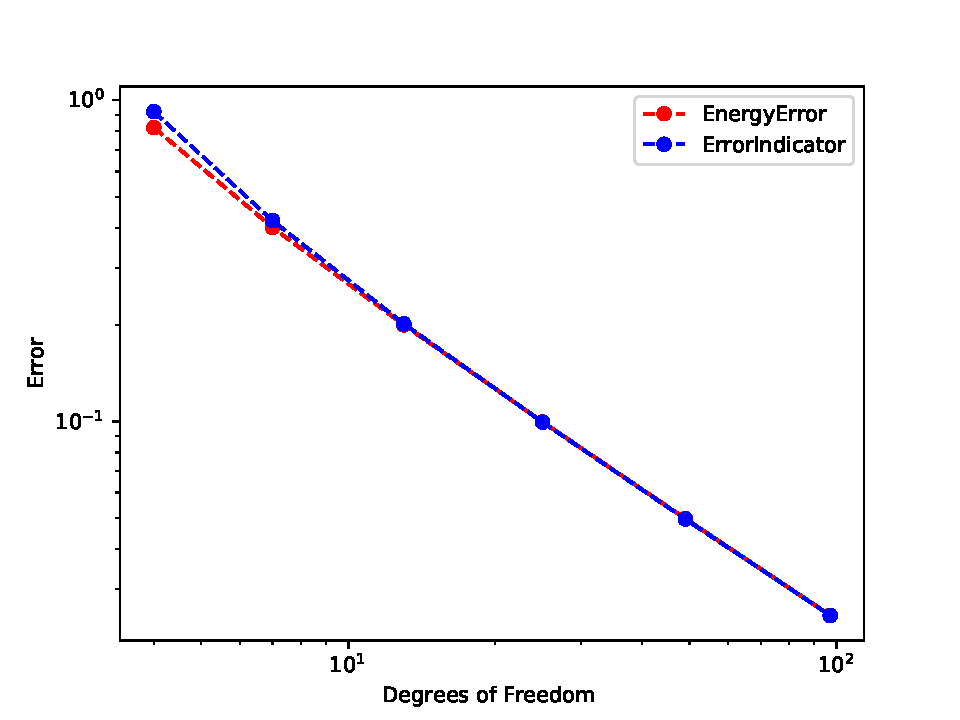
\includegraphics[width=0.5\textwidth]{IndicatorElipticPDE_CAM.pdf}
   
 \label{fig:IndicatorEllipticalCAM}
\end{figure}

We have argued thus far numerically and otherwise that our indicator $\eta$ is a measure of the true error in an elliptic PDE. This dissertation however concerns space adaptation in parabolic PDEs. We therefore must extend our logic slightly to include the parabolic case.
It may be noted that in problem \ref{prob:weak2} we look for a solution of the form $u(\cdot , t)$ where the function $u$ lives on some specific time $t$. So intuitively it seems that an error indicator based on the gradient may work equally well in this time dependent setting. In fact in problem \ref{prob:weak2} when spacial components are discretised with the FEM and give rise to the bilinear functional $a(u, v)$ which is the same as the one that arises in our elliptical problem \ref{eq:Steady Diffusion2}.


\begin{figure}
With this justification in mind we investigate numerically the effectivity indexes in some of our parabolic model problems. Below we see the results of \ref{eq:Simple Heat1}.  
\begin{center}
  \begin{tabular}{r|cccccc}  \label{table:IndicatorPDE1}
    $Mesh$   & DOFs & $\|u-u_h\|_{a(0,1)}$ & $\eta$ & Effectivity Index  \\ \hline
    $1$ & $4$ & 1.63002 &  1.71983  &  1.05501\\
    $2$ & $7$ & 0.862629 &  0.878275 & 1.018138 \\
    $3$ & $13$ & 0.435436 & 0.43934  & 1.008966  \\
	$4$ & $25$ & 0.218313 &  0.219703  &1.006367\\
    $5$ & $49$ & 0.109433 &  0.109858 & 1.003884 \\
    $6$ & $97$ & 0.0548128 &  0.0549298  & 1.002135\\
  \end{tabular}
\end{center}

\caption{The error indicator convergences uniformly to the true solution and is always larger than it}
   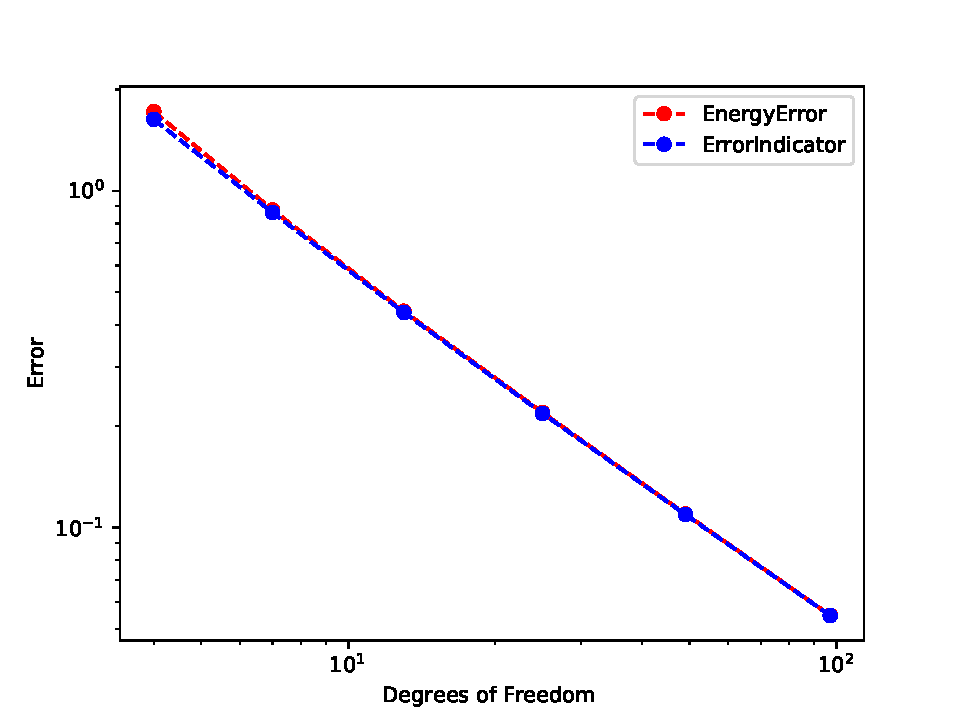
\includegraphics[width=0.5\textwidth]{IndicatorPDE1.pdf}
   
 \label{fig:IndicatorPDE1}
\end{figure}


\begin{figure}[h]
We now compare the above results for \ref{eq:Simple Heat1} to our results for our other parabolic model problem \ref{eq:Simple Heat2}. 
\begin{center}
  \begin{tabular}{r|cccccc}  \label{table:IndicatorPDE2}
    $Mesh$   & DOFs & $\|u-u_h\|_{a(0,1)}$ & $\eta$ & Effectivity Index  \\ \hline
    $1$ & $4$ & 0.29131 &  0.108467  & 0.372342 \\
    $2$ & $7$ & 0.074447 &  0.0201663  &  0.270881\\
    $3$ & $13$ & 0.0229916 & 0.0135003  & 0.587184 \\
	$4$ & $25$ & 0.00855775 &  0.00718688  & 0.8398095 \\
    $5$ & $49$ & 0.00381445 &  0.00363495  & 0.9529421  \\
    $6$ & $97$ & 0.00184453 &  0.00182187   &  0.9877150\\
  \end{tabular}
\end{center}


\caption{Here we have some interesting interaction between the $\eta$ and the true error. The error indicator converges from below and sharply at first. This may present a problem for a self-adapting code specifically with regards to coarsening of a mesh. It may be necessary to add some exceptions to maintain a minimum number of DOFs obviously at least two, but possibly more where necessary}
   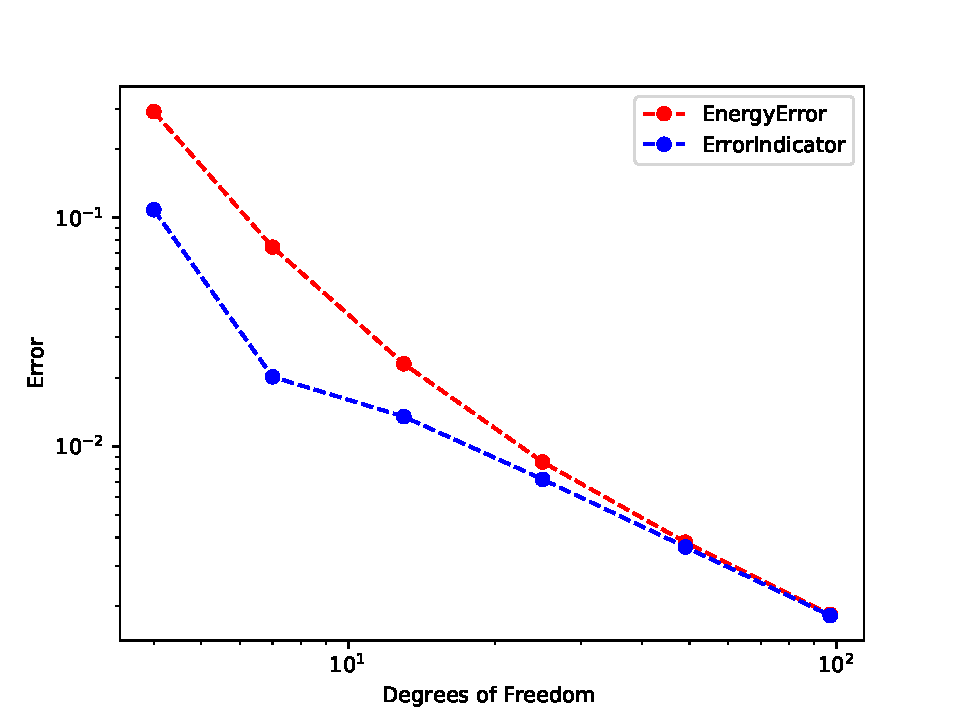
\includegraphics[width=0.5\textwidth]{IndicatorPDE2.pdf}
   
 \label{fig:IndicatorPDE2}
\end{figure}

\clearpage

\subsection{Implementation} \label{subsubsec:KK Implementation}

To make the most use of our existing member functions in the SpaceMesh class we should make sure our gradient recovery vector match the space nodes. This will allow the interpolant to be completely defined by the new vector and a reference to a grid. This means that the first and last point though should be defined on the boundary. In practise this means extrapolating the line segment in the final interval on each side to the boundary and taking its value there. A function which does this is included for illustration in appendix \ref{app:Gradient Recovery}.






\newpage

\section{Design of Adaptive Algorithms} \label{sec:Adaptive}

The purpose of adaptive FEM techniques can be thought of in different ways. It is not simply the case that adding nodes where there are large errors will lead to a "better" solution in any common sense way. It does however have interesting implications for the design for error analysis and the design of scientific software. Possible advantages include:

\begin{enumerate}
\item Equidistributed errors may serve certain applications better for example if we are studying the effects of changing parameters. 

\item If adaptivity is found to be effective we may be able to achieve a comparable quality of solution with the same or fewer degrees of freedom. This would save valuable computing resources if we need to run our code multiple times or for large matrix systems. 

\item The choice of mesh, initial set-up notwithstanding, is selected automatically by the algorithm. This limits the calibration needed by the end user and so allows for a professional finish on a software package for the FEM. 
\end{enumerate}

The rest of this chapter will describe an algorithm that can achieve the equidistribution of the errors in space. Then we will explore the implementation in principle and in practice. In subsection \ref{subsubsec:CMR} we reflect on how we have been implementing the Implicit Euler thus far and explore the methodology that will allow us to both refine and coarsen our mesh between time steps. In subsection \ref{subsec:Space Adaptive} we introduce the algorithm for space adaptation. In subsection \ref{subsec:Refine and Coarsen} we look at how the decision to refine and coarsen is taken in the code.  


\subsection{Common Mesh Refinement} \label{subsec:CMR}

Consider the equation \ref{eq:Simple Heat1} and its fully discrete form defined on a suitable mesh $\Omega^{\Delta t}_h$

\begin{align*}
( u_h^{m+1}, \, v_h)  + \: \Delta t a(u_h^{m+1}, v_h) \quad&=\quad (u_h^{m}, \, v_h )  \\
(u^{0}_h) \quad  &= \quad (u_0, v_h) 
\quad \forall v_h \in V \quad \quad 0 \leq m \leq M-1 \\
\end{align*}

Here,
\begin{equation*}
 a(w, v)  = \int_0^L  w' v'  dx \quad \quad (w, v) = \int_0^L  w v  dx
\end{equation*}
 

The right hand side for a non-changing mesh is fairly straightforward calculation as $u_h^{m-1}$ and $v_h$ are both piecewise linear and defined on the same mesh. All we need to do in this case is use quadrature with our test function over each interval or, as we have done, use the mass matrix multiplied by the previous solution $Mu_h^{m-1}$ as explained in \cite{larson2013finite}. 

However, when the mesh evolves from time to time the mass matrix method is no longer meaningful and the integral $(u_h^{m}, \, v_h )$ becomes more difficult to evaluate. To do this we must consider the mesh where $v_h$ is defined which is here the mesh at time $m+1$ and we must consider that the two functions $u_h^{m}$ and $v_h $ are piecewise linear and so we must be careful when using quadrature across the element boundaries on either mesh.


\begin{figure}[h!]
\caption{Approximation to u at time m}
\begin{center}
\begin{tikzpicture} 
\draw[thick,->] (-0.5,0) -- (-0.5,4);
\draw[thick] (-0.5,0)--(0,0) -- (0.25,-0.25) -- (0.5,0.25) --(0.75,0)--(8,0) -- (8.25,-0.25) -- (8.5,0.25) --(8.75,0) -- (10,0) node[anchor=north west]{};

\draw (0.5, 1.5) -- (3,2) -- (4,1.5)--(6, 2.5) -- (7.5, 1.5);


\filldraw (3,0) circle (2pt) node[anchor=north] {$x_{i-1}$};
\filldraw (4,0) circle (2pt) node[anchor=north] {$x_{i}$};
\filldraw (6,0) circle (2pt) node[anchor=north] {$x_{i+1}$};

\draw (10 cm,1pt) -- (10 cm,-1pt) node[anchor=north] {$x_N$};

\end{tikzpicture}
\end{center}
\end{figure}

\begin{figure}[h!]
\caption{Basis function a time m+1}
\begin{center}
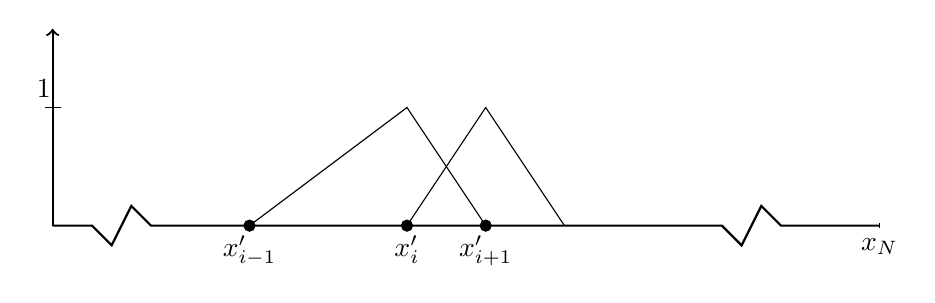
\begin{tikzpicture}
\draw[thick,->] (-0.5,0) -- (-0.5,2.5);
\draw (-0.6,1.5) -- (-0.4,1.5) node[anchor=south east] {$1$};
\draw[thick] (-0.5,0)--(0,0) -- (0.25,-0.25) -- (0.5,0.25) --(0.75,0)--(8,0) -- (8.25,-0.25) -- (8.5,0.25) --(8.75,0) -- (10,0) node[anchor=north west]{};

%\draw (5,0) -- (6,1.5)--(7.5, 0.5);
\draw (4,0) -- (5,1.5)--(6, 0);
\draw (2,0) -- (4,1.5)--(5, 0);
%\draw (0.75,0.5) -- (2,1.5)--(4, 0);


\filldraw (2,0) circle (2pt) node[anchor=north] {$x'_{i-1}$};
\filldraw (4,0) circle (2pt) node[anchor=north] {$x'_{i}$};
\filldraw (5,0) circle (2pt) node[anchor=north] {$x'_{i+1}$};


\draw (10 cm,1pt) -- (10 cm,-1pt) node[anchor=north] {$x_N$};

\end{tikzpicture}
\end{center}
\end{figure}

\begin{figure}[h!] 
\begin{center}
\begin{tikzpicture}
\draw[thick,->] (-0.5,0) -- (-0.5,2.5);
\draw (-0.6,1.5) -- (-0.4,1.5) node[anchor=south east] {$1$};
\draw[thick] (-0.5,0)--(0,0) -- (0.25,-0.25) -- (0.5,0.25) --(0.75,0)--(8,0) -- (8.25,-0.25) -- (8.5,0.25) --(8.75,0) -- (10,0) node[anchor=north west]{};


\filldraw (2,0) circle (2pt) node[anchor=north] {$x''_{i-2}$};
\filldraw (3,0) circle (2pt) node[anchor=north] {$x''_{i-1}$};
\filldraw (4,0) circle (2pt) node[anchor=north] {$x''_{i}$};
\filldraw (5,0) circle (2pt) node[anchor=north] {$x''_{i+1}$};
\filldraw (6,0) circle (2pt) node[anchor=north] {$x''_{i+2}$};



\draw (10 cm,1pt) -- (10 cm,-1pt) node[anchor=north] {$x_N$};

\end{tikzpicture}
\end{center}

\caption{A common mesh}
\label{fig:common mesh}
\end{figure}

A safe way to implement $(u_h^{m}, \, v_h )$ is to loop the quadrature with reference to a common mesh like the one in figure \ref{fig:common mesh}. To accomplish this we notice that a common mesh is simply an instance of a the meshes we have previously designed and so we will need a new object from our SpaceMesh class. Then we need some new methods.


\begin{lstlisting}[language=C++]
class SpaceMesh
{
public:
    void CommonMesh( SpaceMesh& firstmesh, SpaceMesh& secondmesh );
    void Range( double lowerlimit, double upperlimit, 
    std::vector<double>& Nodes);
    double TestFunctions(int nodeIndex, double x);
    };
\end{lstlisting}

The CommonMesh method is a simple "copy erase if" algorithm made easy by the utilities in the <algorithm> library in C++11 or later. Called on our new instance of SpaceMesh it creates the common mesh required for reference. 

The Range method will return all the nodes within a given range as a dynamic array. This is a design choice rather than a necessity. We choose to create an outer loop over our mesh in the current time then an inner loop which loops over the common mesh to see how many subintervals to choose. Therefore Range will be called on the common mesh object.

We can create a method TestFunctions which can be called at the current time. Then for every interval in the current mesh object we have a hat function and also our outer loop can be used as the index for said hat function.

We will also need to utilise our interpolating function with a reference to the mesh at the previous time to interpolate the previous solution. 

Clearly this and all the methods thus far mentioned are straight forward to test independently.Once reliability of the code is established we we can create the method needed to build $(u_h^{m}, \, v_h )$. This can be simply described as the test function and previous solution meeting on the common mesh and the quadrature quadrature being carried out there. Two methods which when used together can do this are given for illustration in \ref{app:RHS}

\begin{lstlisting}[language=C++]
void AdaptiveHeatEquation::BuildRHS()
{
mpRHS.clear();
std::vector<double> intervals;
	//create the common mesh from the two earlier ones
refinedsmesh.CommonMesh(mpsmesh, oldmesh);
double integral;
	//loop over internal nodes ignoring half hats for now
for (int i = 1; i<mpsmesh.meshsize(); i++)
{
    integral=0;
    	//read the common mesh intervals contained 
    refinedsmesh.Range(mpsmesh.ReadSpaceNode(i-1), 
    mpsmesh.ReadSpaceNode(i+1), intervals);
		//loop over contained intervals
    for(int j = 0; j<intervals.size()-1; j++)
    {
        integral = integral + IntegrateBasisWithU(i, intervals.at(j),
                    intervals.at(j+1));
    }
    	//save the results of integration on interval on current mesh 
    mpRHS.push_back(integral);
}
}
\end{lstlisting} 

\subsection{Space Adaptivity} \label{subsubsec:Space Adaptive}

In the previous section we described an a posteriori error indicator derived from post processing the gradient of our approximation. This indicator the possibility of adapting the space mesh of our Finite Element Method either manually or algorithmically during implementation. In fact, our specific error indicator is one of the first initially introduced for this purpose by \cite{babuska1978posteriori} although it was derived and explained differently there \cite{ainsworth65001posteriori}.

The algorithm for a parabolic problem consists of:


\begin{algorithm}
\begin{algorithmic} 
\FORALL{Time steps}
\STATE calculate $u_h$
\STATE calculate the error indicator
\STATE save the elements that are too large or small
\STATE refine and coarsen
\ENDFOR
\end{algorithmic}
\end{algorithm}

An efficient way of doing this is adding some utility methods to our SpaceMesh class which allow us to insert and remove nodes from an array. We add a set of methods to our Solver class for calculating and comparing the error indicators to the tolerances. We can make our code read similar to above. 


\begin{lstlisting}[language=C++, label=code:adaptive_solver] 
for(int j = 0; j<mptimemesh.NumberOfTimeSteps(); j++)
{
    BuildSystemAtTimeStep();
    SystemSolver();
    mpPreviousSolution = mpx;

    SaveIntervalsForRefinement();
    SaveIntervalsForCoarsening();
    mpsmesh.BisectIntervals(intervalsForRefinement);
    mpsmesh.CoarsenIntervals(NodesForRemoval);
}
\end{lstlisting}



\subsection{Refining and coarsening} \label{subsec:Refine and Coarsen}

In practise there are still technical details and design decisions involved in making the above code run. These decisions are often brushed over or taken for granted in the literature. This seemed a little odd to us as we saw many possible ways of both refining and of coarsening a mesh based on reliable a posteriori data. These different choices would lead to different outcomes and different challenges in the software. 
Of the two processes refinement is clearly the simpler one. Our implementation simply compares the error indicator over each element to a tolerance and if the $\eta > tolerance$ then we bisect the interval.


\subsubsection{Coarsening} \label{subsubsec:Coarsening}

Coarsening is less straightforward. Most approaches to this problem will not be able to be applied on the boundary interval in the same way. We experimented with several ways of doing this


\begin{enumerate}
\item Take the norm of the error indicator across two elements and remove the middle node if that value is below a tolerance. This is method depends on some consistency in the error distribution but does yield safe code without worries about the unexpected loss of nodes.

\item Take the error indicator over each element and then if below a certain tolerance remove both associated nodes and bisect the interval. This effectively redistributes the error however it needs exceptions on the boundary and can lead to some very difficult to debug code.

\item Do as above but simply remove one of the nodes i.e. always the upper or lower. This can be written in such a way as to avoid the boundaries and ugly exception lists. Also, even if the decision is sub-optimal for small enough step size $ \Delta t$ the refinement method should handle it quickly.

\item Once again do as above but compare the errors over the elements to the left and right and take the node separating the smaller two. This is possibly the neatest solution but still needs exceptions on the boundaries.
\end{enumerate}

In fact there is no reason to restrict yourself to one or another of the methods. A useful feature of the modular code presented in \ref{code:adaptive_solver} is that we can trade different coarsening methods in and out as we like. In fact we implement the final method for the production of our numerical experiments.

A final note on coarsening which we touched on in the caption to figure \ref{fig:IndicatorPDE2} is one of rapid hollowing out of a mesh. For our model problem \ref{eq:Simple Heat2} the error indicator is smaller than the true error. This is exacerbated by the fact that $u_h$ has large changes in gradient in its initial conditions but then in the final time is almost a linear function. This leads to a situation where at some time step the coarsening function removes all but the boundary nodes and typically this happens instantly. When initially implemented our solver was not robust enough to handle only one element at a time step. 
This issue needs to be considered carefully and in advance of implementation to avoid spending large amounts of time re-writing code or finding ways around.

\clearpage

\section{Some Numerical Examples} \label{sec:Examples}

\begin{figure}[h!]
\begin{minipage}{0.49\hsize}
   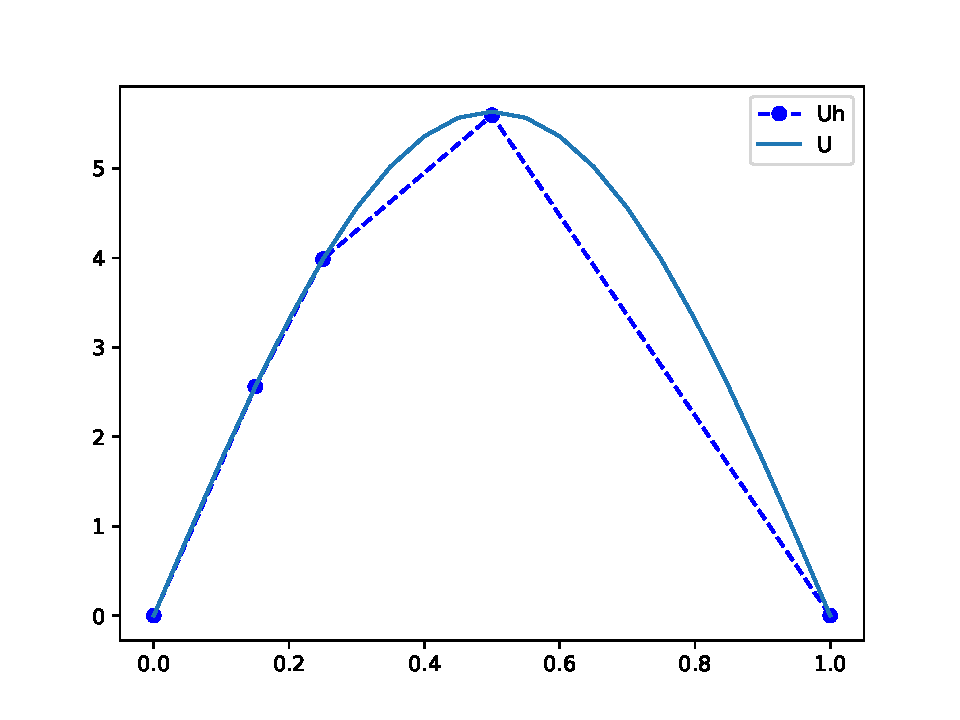
\includegraphics[width=1.1\textwidth]{adap1_time_1.pdf}
  \end{minipage}
  \hfill
    \begin{minipage}{0.49\hsize}
    \vspace{5mm}
    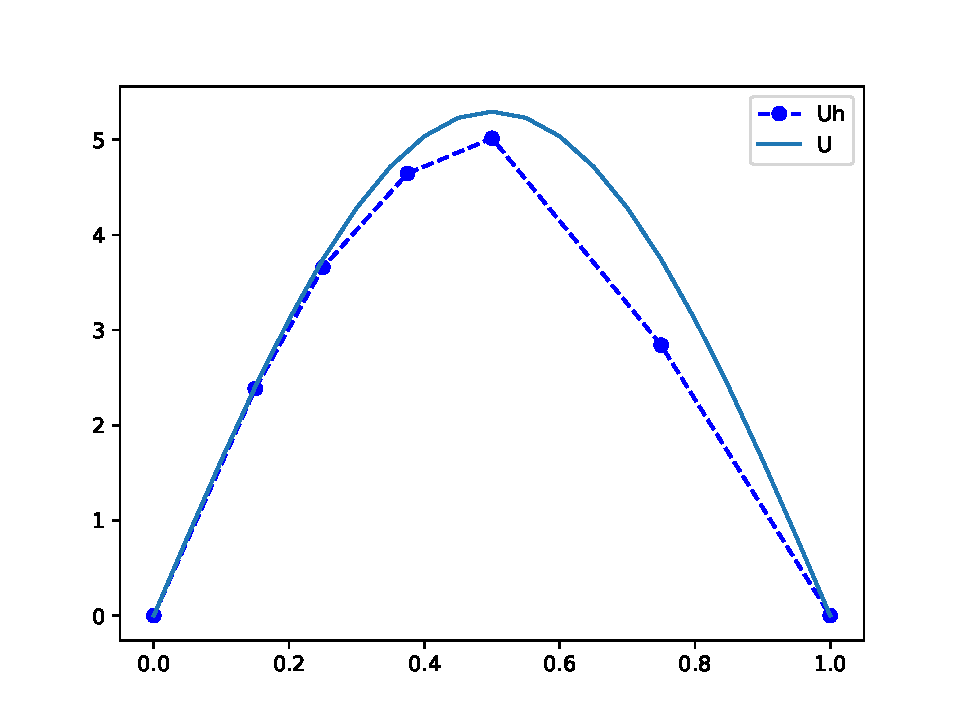
\includegraphics[width=1.1\textwidth]{adap1_time_2.pdf}
  \label{fig:c}
\end{minipage}
    \end{figure}
    

\begin{figure}[h!]
\begin{minipage}{0.49\hsize}
   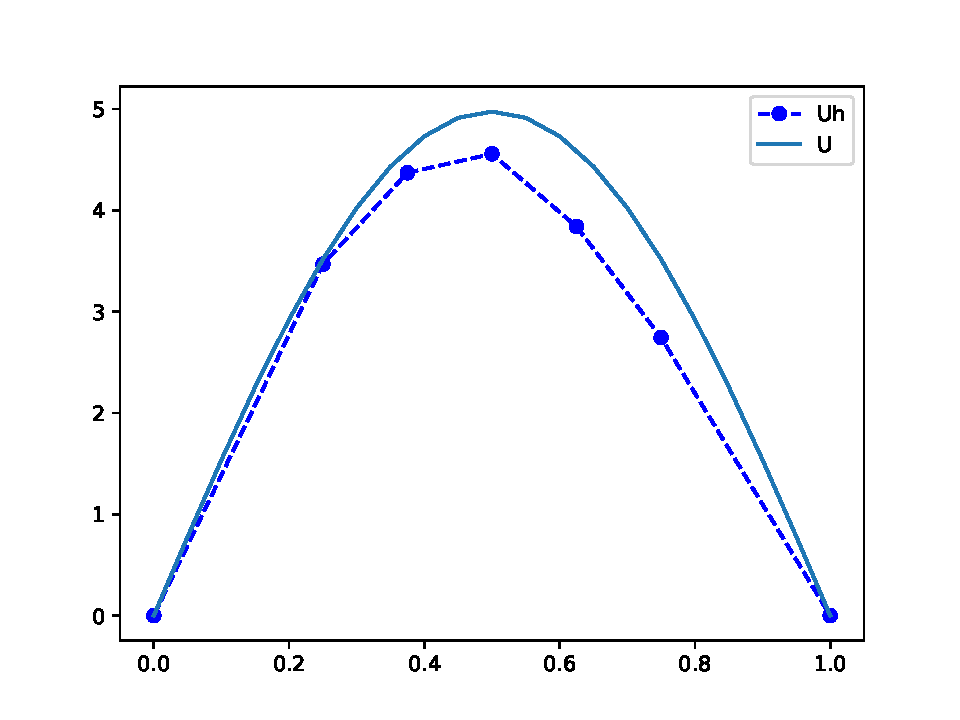
\includegraphics[width=1.1\textwidth]{adap1_time_3.pdf}
  \end{minipage}
  \hfill
    \begin{minipage}{0.49\hsize}
    \vspace{5mm}
    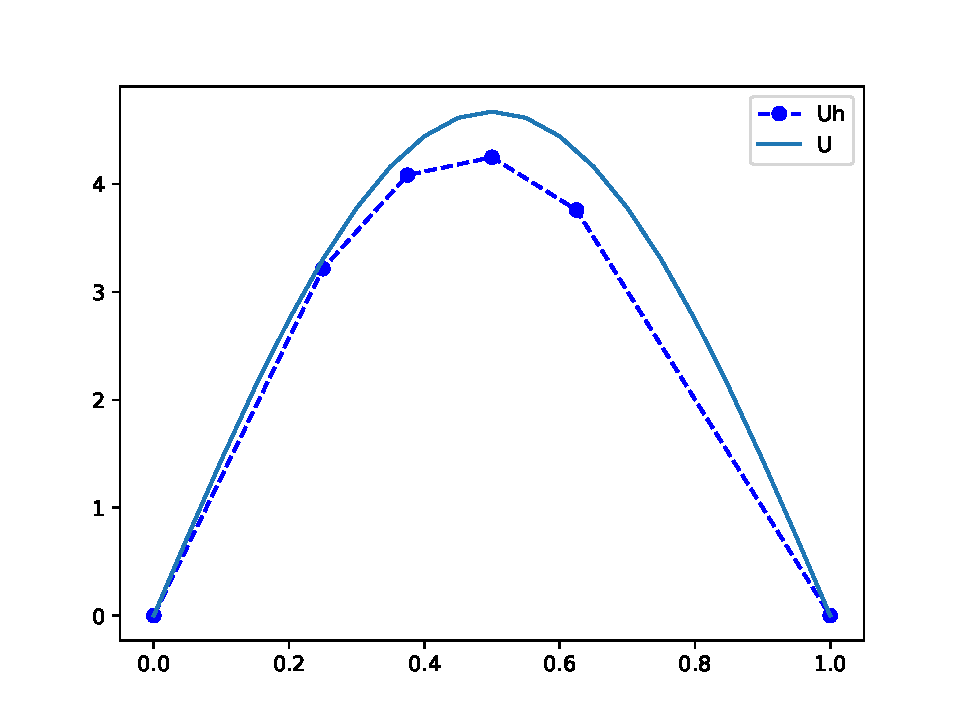
\includegraphics[width=1.1\textwidth]{adap1_time_4.pdf}
  \label{fig:c}
\end{minipage}
    \end{figure}

\begin{figure}[h!]
   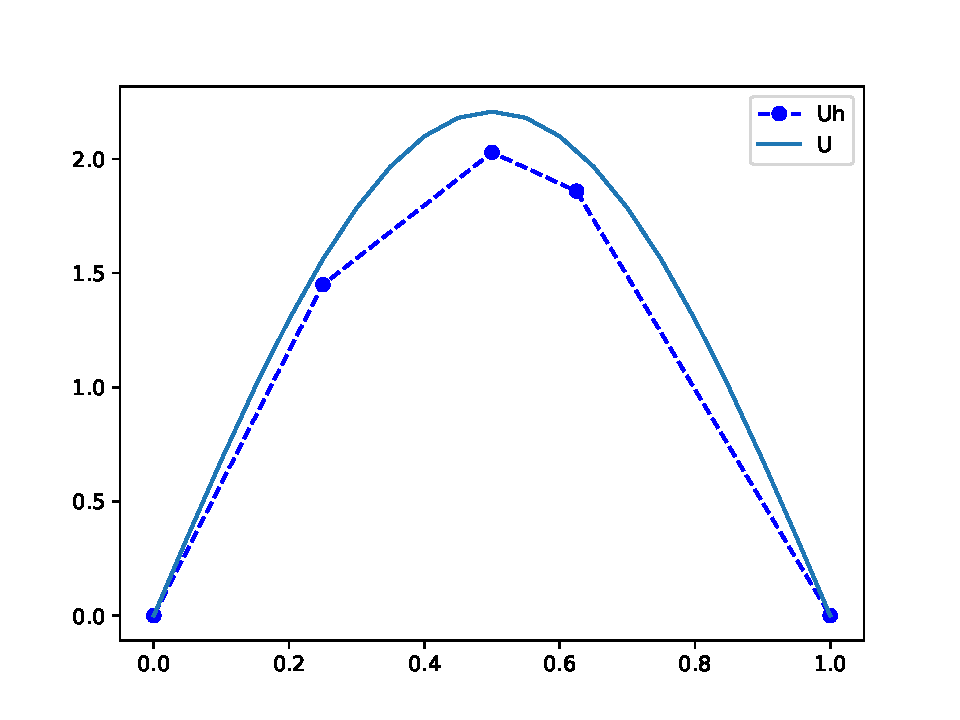
\includegraphics[width=0.5\textwidth]{adap1_time_16.pdf}
   
 \label{fig:IndicatorPDE1}
\end{figure}

\clearpage

\subsection{A More challenging PDE} \label{subsec:time dep boundaries }

For the purposes of testing our adaptive FEM code more extensively we will define a PDE with regions of steeper gradient and more unpredictable behaviour. To do this we implement time dependent boundary conditions.

\begin{subequations} 
\begin{align}\label{eq:time dep boundaries}
  \dot{u} - \pi^{-2} \: u'' = &\: 0 \quad x \in [0, L], \quad t \in (0, 1] \\ 
  u(0, t) & = t  \quad u(1, t) = e^{-t} \\
  u(x, 0) & =  2sin(2 \pi x) +x
\end{align}
\end{subequations}


\begin{figure}[h!]
   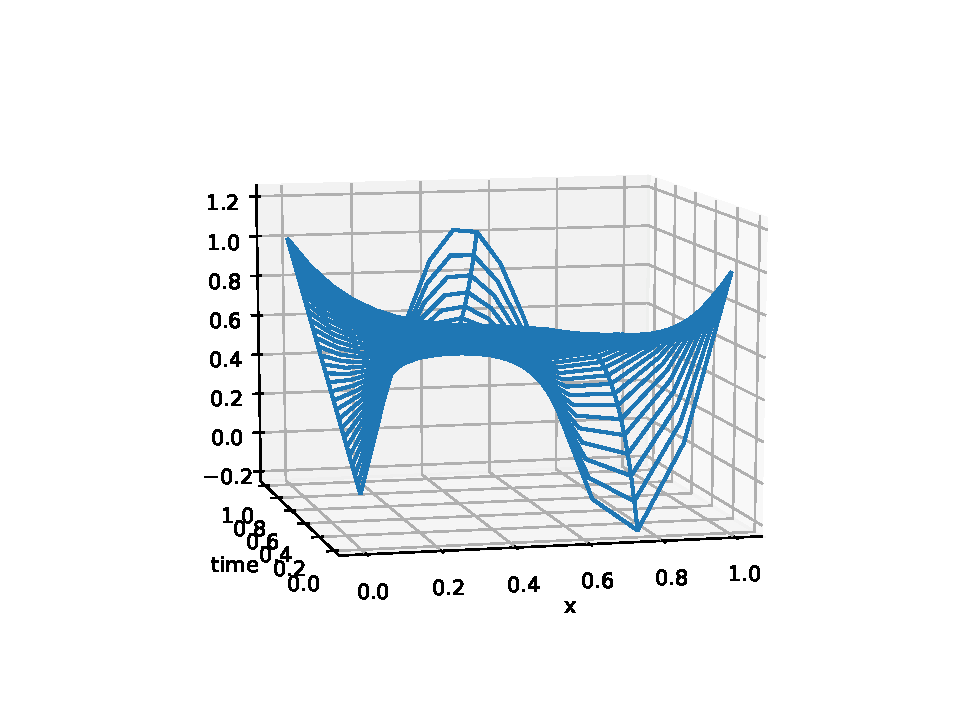
\includegraphics[width=0.9\textwidth]{TestFixedMesh.pdf}
   
 \label{fig:IndicatorPDE1}
\end{figure}

\newpage


\section{Conclusions} \label{sec:conclusions}

To be decided

\newpage

\appendix

\section{Lax Milgram} \label{app:LM}

\begin{theorem}[Lax Milgram]
%\label{Lax Milgram}
Let V be a real Hilbert Space with associated norm $\|\dot{•}\|$. Also let $a(\dot{•}, \dot{•})$ be a bilinear functional on V x V with:

(a) $a(\cdot, \cdot)$ is coercive, i.e. there exists a positive constant $c_0 \forall v \in V |a(v, v)|  \geq c_0 \|v\|^2_V$ 

(b) $a(\cdot, \cdot)$ is continuous i.e. there exists a positive constant $c_1 \forall v, w \in V |a(v, w) \leq c_1 \|v\|_V \|w\|_V$ 

and for $\ell(\cdot)$ a bilinear functional also on V such that 

(c) $\ell(\cdot)$ is continuous i.e. there exists a positive constant $c_2 \forall v \in V |\ell(\cdot)|  \leq c_2 \|v\|_V$

Then there $\exists u \in V: a(u, v) = \ell(v) \forall v \exists V$ and u is unique.
\end{theorem}

\section{Tridiagonal Matrices} \label{app:Tridiag}

\begin{lstlisting}[language=C++]
class TriDiagMatrix
{
public:
    void MatrixSolver( std::vector<double> f, std::vector<double> &x )
    
protected:
    std::vector<double> mpDiagonal;
    std::vector<double> mpLowerDiag;
    std::vector<double> mpUpperDiag;
};
    
    void TriDiagMatrix::MatrixSolver( std::vector<double> f,
     std::vector<double> &x )
    {
        std::vector<double> cDiagonal = mpDiagonal;
        std::vector<double> cLowerDiag = mpLowerDiag;
        std::vector<double> cUpperDiag = mpUpperDiag;
        x.assign(mpn, 0.);
         //scaling matrix entries
    for(int i=1; i<mpn; i++)
    {
        cDiagonal.at(i) = cDiagonal.at(i)-
        (cUpperDiag.at(i-1)*cLowerDiag.at(i)/cDiagonal.at(i-1));
        f.at(i) = f.at(i)-(f.at(i-1)*cLowerDiag.at(i)/cDiagonal.at(i-1));
    }

        //solving through elimination
     x.at(mpn-1)=f.at(mpn-1)/cDiagonal.at(mpn-1);
     for(int i=mpn-2; i>=0; i=i-1)
     {
         x.at(i) = (f.at(i) - cUpperDiag.at(i)*x.at(i+1))/(cDiagonal.at(i));
     }
    }

\end{lstlisting}

\section{Stiffness Matrix} \label{app:Stiff}

\begin{lstlisting}[language=C++]

class StiffnessMatrix: public TriDiagMatrix
{
public:

    void BuildStiffnessMatrix ( SpaceMesh smesh );
    void BuildGeneralStiffnessMatrix ( SpaceMesh smesh );
    void SetParameters (double k_0, double k_L, double constant);

protected:
    const double M_PI = 2*acos(0);
    double a, mpk_0, mpk_L;
};

void StiffnessMatrix::BuildGeneralStiffnessMatrix ( SpaceMesh smesh )
{
mpn = smesh.meshsize()+1;
mpDiagonal = { a*pow(smesh.ReadSpaceMesh(0), -1)+mpk_0 };
mpLowerDiag = {0};
mpUpperDiag = { -1*a*pow( smesh.ReadSpaceMesh(0), -1 ) };

for(int i=0; i<mpn-2; i++)
    {
        mpDiagonal.push_back( a*pow(smesh.ReadSpaceMesh(i), -1) + 
        a*pow(smesh.ReadSpaceMesh(i+1), -1) );
        mpLowerDiag.push_back( -1*a*pow(smesh.ReadSpaceMesh(i),-1)  );
        mpUpperDiag.push_back( -1*a*pow(smesh.ReadSpaceMesh(i+1), -1) );
    }

mpDiagonal.push_back( a*pow(smesh.ReadSpaceMesh(mpn-2), -1)+mpk_L );
mpLowerDiag.push_back( -1*a*pow(smesh.ReadSpaceMesh(mpn-2),-1) );
mpUpperDiag.push_back( 0 );
}

\end{lstlisting}

\section{Mass Matrix} \label{app:Mass}

\begin{lstlisting}[language=C++]
class MassMatrix: public TriDiagMatrix
{
public:
    void BuildMassMatrix ( SpaceMesh smesh );
    void BuildGeneralMassMatrix ( SpaceMesh smesh );
};

void MassMatrix::BuildGeneralMassMatrix ( SpaceMesh smesh )
{
mpn = smesh.meshsize()+1;
mpDiagonal = {smesh.ReadSpaceMesh(0)*pow(3,-1)};
mpLowerDiag = {0};
mpUpperDiag = {(smesh.ReadSpaceMesh(0)*pow(6,-1))};

for(int i=0; i<mpn-2; i++)
    {
        mpDiagonal.push_back( (smesh.ReadSpaceMesh(i)+
        smesh.ReadSpaceMesh(i+1))*pow(3,-1) );
        mpLowerDiag.push_back( smesh.ReadSpaceMesh(i)*pow(6,-1) );
        mpUpperDiag.push_back( smesh.ReadSpaceMesh(i+1)*pow(6,-1) );
    }

mpDiagonal.push_back( smesh.ReadSpaceMesh(mpn-2)*pow(3,-1)) ;
mpLowerDiag.push_back( smesh.ReadSpaceMesh(mpn-2)*pow(6,-1) );
mpUpperDiag.push_back( 0 );
}

\end{lstlisting}

\section{Space Mesh} \label{app:space mesh}

\begin{lstlisting}[language=C++]
class SpaceMesh
{
public:
    void Range( double lowerlimit, double upperlimit, 
    std::vector<double>& Nodes);
    void CommonMesh( SpaceMesh& firstmesh, SpaceMesh& secondmesh );
    double TestFunctions(int nodeIndex, double x);


protected:
    std::vector<double> mpSpaceNodes;
};

void SpaceMesh::Range( double lowerlimit, double upperlimit, 
		std::vector<double>& Nodes)
{
    Nodes.clear();
    for(auto i:mpSpaceNodes)
        if(lowerlimit<=i&&i<=upperlimit)
        {
            Nodes.push_back(i);
        }
}

void SpaceMesh::CommonMesh( SpaceMesh& firstmesh, SpaceMesh& secondmesh )
{
    mpSpaceNodes=firstmesh.mpSpaceNodes;
    mpSpaceNodes.insert( mpSpaceNodes.end(),
    secondmesh.mpSpaceNodes.begin(), secondmesh.mpSpaceNodes.end() );
    sort(mpSpaceNodes.begin(), mpSpaceNodes.end());
    mpSpaceNodes.erase( unique( mpSpaceNodes.begin(), 
    mpSpaceNodes.end()), mpSpaceNodes.end() );
}

double SpaceMesh::TestFunctions( int nodeIndex, double x)
{
        if((nodeIndex==0)||(nodeIndex==meshsize()))
    {
        return 0;
    }
    else if (x<mpSpaceNodes[nodeIndex]-ReadSpaceMesh(nodeIndex-1)||
    x>mpSpaceNodes[nodeIndex]+ReadSpaceMesh(nodeIndex))
    {
        return 0;
    }
    else if (x<=mpSpaceNodes[nodeIndex])
    {
        return pow(ReadSpaceMesh(nodeIndex-1),-1)*
        (x-mpSpaceNodes.at(nodeIndex))+1;
    }
    else if (x>mpSpaceNodes[nodeIndex])
    {
        return -pow(ReadSpaceMesh(nodeIndex),-1)*
        (x-mpSpaceNodes.at(nodeIndex))+1;
    }
}

\end{lstlisting}


\section{Time Mesh} \label{app:time mesh}

\begin{lstlisting}[language=C++]
class TimeMesh
{
public:

    void CopyTimeMesh (const TimeMesh& oldTimeMesh);
    void GenerateTimeMesh ( std::vector<double> TimeNodes );
        //takes mTimeStep which is one less than the number of
        //nodes and a Final time and produces the nodes i.e. m+1 equal steps
    void GenerateUniformTimeMesh ( int mTimeSteps, double TFinalTime );
    void BisectInterval (int lowerIndex, int upperIndex);
    void GloballyBisectTimeMesh ();
    void InsertTimeNode ( double ti );
    void RefreshTimeMesh();
    void PrintTimeNodes ();
    void PrintTimeMesh ();
    double ReadTimeStep (int i);
    	//reads the step size between nodes
    double ReadTimeMesh (int i);
    int NumberOfTimeSteps();
protected:
std::vector<double> mpTimeNodes;
};

\end{lstlisting}

\section{PDE Interface} \label{app:PDE Interface}

\begin{lstlisting}[language=C++]
class APDE
{
    public:
        friend class GeneralHeat;
        virtual double ContinuousAnalyticSolution( double x, double t );
        virtual double AnalyticGradientWRTx( double x, double t );
        virtual double EllipticalRHSfunction( double x );
        virtual double FirstBoundary( double t );
        virtual double SecondBoundary( double t );
        virtual void InitialCondition ( SpaceMesh& a_mesh, 
        std::vector<double>& first_U );
    protected:
        const double M_PI = 2*acos(0);
        double a, g_0, g_L, k_0, k_L;
};
\end{lstlisting}

\section{A Parabolic PDE} \label{app:PDE Interface}

\begin{lstlisting}[language=C++]

class Test: public APDE
{
    public:
        friend class GeneralHeat;
        void InitialCondition ( SpaceMesh& a_mesh, 
        std::vector<double>& first_U );
        double FirstBoundary( double t );
        double SecondBoundary( double t );
        Nonanalytic( );
};

double Test::FirstBoundary( double t ){ return t; }

double Test::SecondBoundary( double t ){ return exp(-t); }

void Test::InitialCondition ( SpaceMesh& a_mesh, std::vector<double>& first_U )
{
    first_U.clear();
    double var;
    for (int i = 0; i<a_mesh.meshsize()+1; i++)
    {
        var = sin(2*M_PI*a_mesh.ReadSpaceNode(i))+a_mesh.ReadSpaceNode(i);
        first_U.push_back(var);
    }
}

Test::Nonanalytic( )
{
    a= 0.1, g_0 =0 , g_L = 1, k_0 = pow(10, 300), k_L = pow(10, 300);
}
\end{lstlisting}

\section{PDE Interface} \label{app:PDE Interface}

\begin{lstlisting}[language=C++]
class APDE
{
    public:
        friend class GeneralHeat;
        virtual double ContinuousAnalyticSolution( double x, double t );
        virtual double AnalyticGradientWRTx( double x, double t );
        virtual double EllipticalRHSfunction( double x );
        virtual double FirstBoundary( double t );
        virtual double SecondBoundary( double t );
        virtual void InitialCondition ( SpaceMesh& a_mesh, 
        std::vector<double>& first_U );
    protected:
        const double M_PI = 2*acos(0);
        double a, g_0, g_L, k_0, k_L;
};
\end{lstlisting}

\section{Gradient Recovery} \label{app:Gradient Recovery}

\begin{lstlisting}[language=C++]
void GeneralHeat::GradientRecoveryFunction( SpaceMesh& relevantMesh,
       std::vector<double>& gradvec, std::vector<double>& gradrecovery ) {
    	
    	//(x_0, y_0) (x_1, y_1) define the line segment to be hard coded
    double x_0 = 0.5*(relevantMesh.ReadSpaceNode(1)+
    				relevantMesh.ReadSpaceNode(0));
    double y_0 = gradvec.at(0);
    double x_1 = relevantMesh.ReadSpaceNode(1);
    double y_1 = 0.5*(gradvec.at(1)+gradvec.at(0));

    gradrecovery.push_back(y_0+(relevantMesh.ReadSpaceNode(0)-
    						x_0)*(y_1-y_0)/(x_1-x_0));
		
		//take the midpoint of the two gradients where undefined
    for(int i = 0; i<relevantMesh.meshsize()-1; i++)
    {
        gradrecovery.push_back(0.5*(gradvec.at(i)+gradvec.at(i+1)));
    }
		
		//the hardcoding needs to happen on both sides
    x_0 = relevantMesh.ReadSpaceNode(mpsmesh.meshsize()-1);
    y_0 = gradrecovery.back();
    x_1 = 0.5*(relevantMesh.ReadSpaceNode(relevantMesh.meshsize())			   
    +relevantMesh.ReadSpaceNode(relevantMesh.meshsize()-1));
    y_1 = gradvec.back();

    gradrecovery.push_back(y_0+
    (mpsmesh.ReadSpaceNode(mpsmesh.meshsize())-x_0)*(y_1-y_0)/(x_1-x_0));
}
\end{lstlisting}

\section{Build RHS} \label{app:RHS}

\begin{lstlisting}[language=C++]
double AdaptiveHeatEquation::IntegrateBasisWithU( 
	int NodeIndex, double lowerlimit, double upperlimit ){
    auto SolutionWithBasis = [&](double x)
        { return mpsmesh.TestFunctions( NodeIndex, x)*
        GeneralInterpolant(x, oldmesh, mpPreviousSolution); };
    return gauss<double, 7>::integrate(SolutionWithBasis, lowerlimit, upperlimit);
	}

void AdaptiveHeatEquation::BuildRHS() {
	refinedsmesh.CommonMesh(mpsmesh, oldmesh);
	double integral;
	for (int i = 1; i<mpsmesh.meshsize(); i++)
	{
    	integral=0;
    	refinedsmesh.Range(mpsmesh.ReadSpaceNode(i-1),
    	 mpsmesh.ReadSpaceNode(i+1), intervals);

    for(int j = 0; j<intervals.size()-1; j++)
    {
        integral = integral + IntegrateBasisWithU(i, 
        intervals.at(j), intervals.at(j+1));
    }
    mpRHS.push_back(integral);
}
}

\end{lstlisting}

\newpage

	\bibliography{References}
	\bibliographystyle{plain}

\end{document}
